%%
% Copyright (c) 2017 - 2022, Ulf Köther;
% Copyright (c) 2017 - 2022, Pascal Wagler;
% Copyright (c) 2014 - 2022, John MacFarlane
%
% All rights reserved.
%
% Redistribution and use in source and binary forms, with or without
% modification, are permitted provided that the following conditions
% are met:
%
% - Redistributions of source code must retain the above copyright
% notice, this list of conditions and the following disclaimer.
%
% - Redistributions in binary form must reproduce the above copyright
% notice, this list of conditions and the following disclaimer in the
% documentation and/or other materials provided with the distribution.
%
% - Neither the name of John MacFarlane nor the names of other
% contributors may be used to endorse or promote products derived
% from this software without specific prior written permission.
%
% THIS SOFTWARE IS PROVIDED BY THE COPYRIGHT HOLDERS AND CONTRIBUTORS
% "AS IS" AND ANY EXPRESS OR IMPLIED WARRANTIES, INCLUDING, BUT NOT
% LIMITED TO, THE IMPLIED WARRANTIES OF MERCHANTABILITY AND FITNESS
% FOR A PARTICULAR PURPOSE ARE DISCLAIMED. IN NO EVENT SHALL THE
% COPYRIGHT OWNER OR CONTRIBUTORS BE LIABLE FOR ANY DIRECT, INDIRECT,
% INCIDENTAL, SPECIAL, EXEMPLARY, OR CONSEQUENTIAL DAMAGES (INCLUDING,
% BUT NOT LIMITED TO, PROCUREMENT OF SUBSTITUTE GOODS OR SERVICES;
% LOSS OF USE, DATA, OR PROFITS; OR BUSINESS INTERRUPTION) HOWEVER
% CAUSED AND ON ANY THEORY OF LIABILITY, WHETHER IN CONTRACT, STRICT
% LIABILITY, OR TORT (INCLUDING NEGLIGENCE OR OTHERWISE) ARISING IN
% ANY WAY OUT OF THE USE OF THIS SOFTWARE, EVEN IF ADVISED OF THE
% POSSIBILITY OF SUCH DAMAGE.
%%
%
% This template is build upon the 'default.latex' template from pandoc:
%
% https://github.com/jgm/pandoc/tree/master/data/templates
%
% Version from: 2022-05-17
%
% Pandoc version: 2.18.1
%
% Additionally, some code was borrowed from the Eisvogel pandoc template
% by Pascal Wagler:
%
% https://github.com/Wandmalfarbe/pandoc-latex-template
%
%
% All changes were applied to build a report- / thesis-template for the HSBA.
%
%%

% Options for packages loaded elsewhere
\PassOptionsToPackage{unicode}{hyperref}
\PassOptionsToPackage{hyphens}{url}
%
\documentclass[
  11pt,
  a4paper,
  twoside]{scrbook}
\usepackage{amsmath,amssymb}
\usepackage[]{cmbright}

\usepackage{setspace}

\usepackage{iftex}
\ifPDFTeX
  \usepackage[T1]{fontenc}
  \usepackage[utf8]{inputenc}
  \usepackage{textcomp} % provide euro and other symbols
\else % if luatex or xetex
  \usepackage{unicode-math}
  \defaultfontfeatures{Scale=MatchLowercase}
  \defaultfontfeatures[\rmfamily]{Ligatures=TeX,Scale=1}
  \setmonofont[Scale=0.9]{Source Code Pro}
\fi
% Use upquote if available, for straight quotes in verbatim environments
\IfFileExists{upquote.sty}{\usepackage{upquote}}{}
\IfFileExists{microtype.sty}{% use microtype if available
  \usepackage[]{microtype}
  \UseMicrotypeSet[protrusion]{basicmath} % disable protrusion for tt fonts
}{}
\makeatletter
\@ifundefined{KOMAClassName}{% if non-KOMA class
  \IfFileExists{parskip.sty}{%
    \usepackage{parskip}
  }{% else
    \setlength{\parindent}{0pt}
    \setlength{\parskip}{6pt plus 2pt minus 1pt}}
}{% if KOMA class
  \KOMAoptions{parskip=half}}
\makeatother
\usepackage{xcolor}
\usepackage[top=30mm,bottom=30mm,left=25mm,right=25mm]{geometry}
\usepackage{color}
\usepackage{fancyvrb}
\newcommand{\VerbBar}{|}
\newcommand{\VERB}{\Verb[commandchars=\\\{\}]}
\DefineVerbatimEnvironment{Highlighting}{Verbatim}{commandchars=\\\{\}}
% Add ',fontsize=\small' for more characters per line
\usepackage{framed}
\definecolor{shadecolor}{RGB}{248,248,248}
\newenvironment{Shaded}{\begin{snugshade}}{\end{snugshade}}
\newcommand{\AlertTok}[1]{\textcolor[rgb]{0.94,0.16,0.16}{#1}}
\newcommand{\AnnotationTok}[1]{\textcolor[rgb]{0.56,0.35,0.01}{\textbf{\textit{#1}}}}
\newcommand{\AttributeTok}[1]{\textcolor[rgb]{0.77,0.63,0.00}{#1}}
\newcommand{\BaseNTok}[1]{\textcolor[rgb]{0.00,0.00,0.81}{#1}}
\newcommand{\BuiltInTok}[1]{#1}
\newcommand{\CharTok}[1]{\textcolor[rgb]{0.31,0.60,0.02}{#1}}
\newcommand{\CommentTok}[1]{\textcolor[rgb]{0.56,0.35,0.01}{\textit{#1}}}
\newcommand{\CommentVarTok}[1]{\textcolor[rgb]{0.56,0.35,0.01}{\textbf{\textit{#1}}}}
\newcommand{\ConstantTok}[1]{\textcolor[rgb]{0.00,0.00,0.00}{#1}}
\newcommand{\ControlFlowTok}[1]{\textcolor[rgb]{0.13,0.29,0.53}{\textbf{#1}}}
\newcommand{\DataTypeTok}[1]{\textcolor[rgb]{0.13,0.29,0.53}{#1}}
\newcommand{\DecValTok}[1]{\textcolor[rgb]{0.00,0.00,0.81}{#1}}
\newcommand{\DocumentationTok}[1]{\textcolor[rgb]{0.56,0.35,0.01}{\textbf{\textit{#1}}}}
\newcommand{\ErrorTok}[1]{\textcolor[rgb]{0.64,0.00,0.00}{\textbf{#1}}}
\newcommand{\ExtensionTok}[1]{#1}
\newcommand{\FloatTok}[1]{\textcolor[rgb]{0.00,0.00,0.81}{#1}}
\newcommand{\FunctionTok}[1]{\textcolor[rgb]{0.00,0.00,0.00}{#1}}
\newcommand{\ImportTok}[1]{#1}
\newcommand{\InformationTok}[1]{\textcolor[rgb]{0.56,0.35,0.01}{\textbf{\textit{#1}}}}
\newcommand{\KeywordTok}[1]{\textcolor[rgb]{0.13,0.29,0.53}{\textbf{#1}}}
\newcommand{\NormalTok}[1]{#1}
\newcommand{\OperatorTok}[1]{\textcolor[rgb]{0.81,0.36,0.00}{\textbf{#1}}}
\newcommand{\OtherTok}[1]{\textcolor[rgb]{0.56,0.35,0.01}{#1}}
\newcommand{\PreprocessorTok}[1]{\textcolor[rgb]{0.56,0.35,0.01}{\textit{#1}}}
\newcommand{\RegionMarkerTok}[1]{#1}
\newcommand{\SpecialCharTok}[1]{\textcolor[rgb]{0.00,0.00,0.00}{#1}}
\newcommand{\SpecialStringTok}[1]{\textcolor[rgb]{0.31,0.60,0.02}{#1}}
\newcommand{\StringTok}[1]{\textcolor[rgb]{0.31,0.60,0.02}{#1}}
\newcommand{\VariableTok}[1]{\textcolor[rgb]{0.00,0.00,0.00}{#1}}
\newcommand{\VerbatimStringTok}[1]{\textcolor[rgb]{0.31,0.60,0.02}{#1}}
\newcommand{\WarningTok}[1]{\textcolor[rgb]{0.56,0.35,0.01}{\textbf{\textit{#1}}}}
\usepackage{longtable,booktabs,array}
\usepackage{calc} % for calculating minipage widths
% Correct order of tables after \paragraph or \subparagraph
\usepackage{etoolbox}
\makeatletter
\patchcmd\longtable{\par}{\if@noskipsec\mbox{}\fi\par}{}{}
\makeatother
% Allow footnotes in longtable head/foot
\IfFileExists{footnotehyper.sty}{\usepackage{footnotehyper}}{\usepackage{footnote}}
\makesavenoteenv{longtable}
\usepackage{graphicx}
\makeatletter
\def\maxwidth{\ifdim\Gin@nat@width>\linewidth\linewidth\else\Gin@nat@width\fi}
\def\maxheight{\ifdim\Gin@nat@height>\textheight\textheight\else\Gin@nat@height\fi}
\makeatother
% Scale images if necessary, so that they will not overflow the page
% margins by default, and it is still possible to overwrite the defaults
% using explicit options in \includegraphics[width, height, ...]{}
\setkeys{Gin}{width=\maxwidth,height=\maxheight,keepaspectratio}
% Set default figure placement to htbp
\makeatletter
\def\fps@figure{htbp}
\makeatother
\setlength{\emergencystretch}{3em} % prevent overfull lines
\providecommand{\tightlist}{%
  \setlength{\itemsep}{0pt}\setlength{\parskip}{0pt}}
\setcounter{secnumdepth}{5}
\newlength{\cslhangindent}
\setlength{\cslhangindent}{1.5em}
\newlength{\csllabelwidth}
\setlength{\csllabelwidth}{3em}
\newlength{\cslentryspacingunit} % times entry-spacing
\setlength{\cslentryspacingunit}{\parskip}
\newenvironment{CSLReferences}[2] % #1 hanging-ident, #2 entry spacing
 {% don't indent paragraphs
  \setlength{\parindent}{0pt}
  % turn on hanging indent if param 1 is 1
  \ifodd #1
  \let\oldpar\par
  \def\par{\hangindent=\cslhangindent\oldpar}
  \fi
  % set entry spacing
    \setlength{\parskip}{#2\cslentryspacingunit+5pt}
   }%
 {}
\usepackage{calc}
\newcommand{\CSLBlock}[1]{#1\hfill\break}
\newcommand{\CSLLeftMargin}[1]{\parbox[t]{\csllabelwidth}{#1}}
\newcommand{\CSLRightInline}[1]{\parbox[t]{\linewidth - \csllabelwidth}{#1}\break}
\newcommand{\CSLIndent}[1]{\hspace{\cslhangindent}#1}
\ifLuaTeX
\usepackage[bidi=basic]{babel}
\else
\usepackage[bidi=default]{babel}
\fi
\babelprovide[main,import]{english}
% get rid of language-specific shorthands (see #6817):
\let\LanguageShortHands\languageshorthands
\def\languageshorthands#1{}
\usepackage{booktabs}
\renewcommand{\textfraction}{0.05}
\renewcommand{\topfraction}{0.8}
\renewcommand{\bottomfraction}{0.8}
\renewcommand{\floatpagefraction}{0.75}
\usepackage[automark,headsepline=0.9pt]{scrlayer-scrpage}
%\usepackage[authordate,backend=biber]{biblatex-chicago}
\newenvironment{abstract}{}{}
\usepackage{abstract}
\usepackage{suffix}
\usepackage{xstring}
\usepackage{relsize}
\usepackage{acronym}
\usepackage{xcolor}
\usepackage{float}
\usepackage{booktabs}
\usepackage{longtable}
\usepackage{array}
\usepackage{multirow}
\usepackage{wrapfig}
\usepackage{float}
\usepackage{colortbl}
\usepackage{pdflscape}
\usepackage{tabu}
\usepackage{threeparttable}
\usepackage{threeparttablex}
\usepackage[normalem]{ulem}
\usepackage{makecell}
\usepackage{xcolor}
\usepackage{siunitx}
\newcolumntype{d}{S[input-symbols = ()]}
\usepackage{caption}
\usepackage{graphicx}
\usepackage{siunitx}
\usepackage{hhline}
\usepackage{calc}
\usepackage{tabularx}
\usepackage{adjustbox}
\usepackage{hyperref}
\ifLuaTeX
  \usepackage{selnolig}  % disable illegal ligatures
\fi

\usepackage{csquotes}
\usepackage{tocloft}

\IfFileExists{bookmark.sty}{\usepackage{bookmark}}{\usepackage{hyperref}}
\IfFileExists{xurl.sty}{\usepackage{xurl}}{} % add URL line breaks if available
\urlstyle{same} % disable monospaced font for URLs
\hypersetup{
  pdftitle={Digital Tool Box -- Project Report},
  pdfauthor={Tania Testperson (XXXX); Max Mustermann (XXXX)},
  pdflang={en},
  hidelinks,
  pdfcreator={LaTeX via pandoc}}

\title{Digital Tool Box -- Project Report}
\usepackage{etoolbox}
\makeatletter
\providecommand{\subtitle}[1]{% add subtitle to \maketitle
  \apptocmd{\@title}{\par {\large #1 \par}}{}{}
}
\makeatother
\subtitle{Project work as part of the Bachelor of Science (B.Sc.) in\\
Media Management \& Communication and Business Informatics}
\author{Tania Testperson (XXXX) \and Max Mustermann (XXXX)}
\date{}


\usepackage{amsthm}
\newtheorem{theorem}{Theorem}[chapter]
\newtheorem{lemma}{Lemma}[chapter]
\newtheorem{corollary}{Corollary}[chapter]
\newtheorem{proposition}{Proposition}[chapter]
\newtheorem{conjecture}{Conjecture}[chapter]
\theoremstyle{definition}
\newtheorem{definition}{Definition}[chapter]
\theoremstyle{definition}
\newtheorem{example}{Example}[chapter]
\theoremstyle{definition}
\newtheorem{exercise}{Exercise}[chapter]
\theoremstyle{definition}
\newtheorem{hypothesis}{Hypothesis}[chapter]
\theoremstyle{remark}
\newtheorem*{remark}{Remark}
\newtheorem*{solution}{Solution}
\begin{document}

%%
%% begin titlepage
%%
\begin{titlepage}
\newgeometry{top=5cm, right=2.5cm, bottom=3cm, left=2.5cm}
\newcommand{\colorRule}[3][black]{\textcolor[HTML]{#1}{\rule{#2}{#3}}}
\begin{flushleft}
\noindent
\\[-1em]
\color[HTML]{000000}
%\makebox[0pt][l]{\colorRule[435488]{1.3\textwidth}{4pt}}
%\par
\noindent

{
	\setstretch{1.4}
	\vfill
		\noindent
	\begin{center}
		
\includegraphics[width=0.6\linewidth]{./01-images/HSBA-Logo-quadratic-version-1.jpg}
	\end{center}
	\vskip 1.5cm
		\begin{center}
		{\huge \textbf{\textsf{Digital Tool Box -- Project Report}}}
	\end{center}
		\vskip 1em
	\begin{center}
		{\Large \textsf{Project work as part of the Bachelor of Science (B.Sc.) in\\
Media Management \& Communication and Business Informatics}}
	\end{center}
		\vskip 2em
	\begin{center}
		{\Large \textsf{Tania Testperson (XXXX)\\Max Mustermann (XXXX)}}
	\end{center}
	\vskip 2em
		\noindent
	\setstretch{1.05}
	\begin{center}
		{\normalsize \textsf{
				\begin{tabular}{ll}
					%% Here you can add any other information you want,
%% as long as it consists of key-value pairs that
%% are separated by an ampersand & and the line ends 
%% with a double backslash: \\

Project Theme & abcde fghij klmno pqrst uvwxyz \\
Study Group & xx \\
Lecturer & ABCDEFG \\
Submitted & \today \\ % erase the '\today' for a hardcoded date like dd.mm.yyyy \\
Team Number & yy \\


										\end{tabular}
\begin{center}
  \textbf{Wordcount was not possible because no tex source}\\
\textbf{file was found -- Rebuild the book with option}\\
\textbf{keep\_tex: yes}
\end{center}

							}}
	\end{center}
		\vfill
}

\textsf{}
\end{flushleft}
\end{titlepage}
\restoregeometry
\pagenumbering{arabic}

%%
%% end titlepage
%%


\pagenumbering{roman}



	\phantomsection
	\addcontentsline{toc}{chapter}{\abstractname}
	\begin{abstract}
	    \doublespacing
		The present specialized bookdown project template you are using now is intended as the basis for a report or thesis at the Hamburg School of Business Administration (HSBA). Compared to the original project template coming with the bookdown package, it generates PDF output only, using a slightly customized LaTeX template based on the original Pandoc-template, which is adapted to the requirements of the HSBA for theses and reports. The main notable differences are an appropriate title page, an automatic word count function, a list of acronyms, an adapted page numbering, the use of the appropriate Chicago Manual of Style citation style (17th edition, CSL-based) and an additional chapter with a basic declaration of honor at the end. In addition, several additional folders are used to demonstrate a basic project structure, as well as a slightly modified file organization to show the use of other R packages in addition to the bookdown basics. The contents of the original bookdown template can be found in the following chapters, the additional code examples in the appendix. For more information about this template, please refer to the file `README.md'.
	\end{abstract}


{
\setcounter{tocdepth}{3}

\phantomsection
\addcontentsline{toc}{chapter}{\contentsname}

\tableofcontents
\newpage
}


\renewcommand{\cftfignumwidth}{6em}
\renewcommand{\cftfigpresnum}{Fig. }
\phantomsection
\addcontentsline{toc}{chapter}{\listfigurename}
\listoffigures
\renewcommand{\cfttabnumwidth}{6em}
\renewcommand{\cfttabpresnum}{Tbl. }
\phantomsection
\addcontentsline{toc}{chapter}{\listtablename}
\listoftables
\newpage

\chapter*{Acronyms}
\addcontentsline{toc}{chapter}{Acronyms}
\begin{acronym}[XXXXX]
% Comment out the examples and define your own acronyms here following this pattern:
%
% \acro{code}[Short Name]{Long Name}
%
% The acronyms must be sorted by hand, they appear in the list of acronyms in the
% order the are listed here.
%
% In the text, then use \ac{code} everywhere in the text where you want to use
% the acronym / abbreviation. When used for the first time, the long name followed
% by the acronym in parenthesis will be inserted, after that the acronym only.
%
% Another example (from the documentation of LaTeX package 'acronym'):
%
% \acro{H2O}[$\mathrm{H_2O}$]{water}
%
% Then \acs{H2O} gets “H2O” and \acl{H2O} prints “water”.
%
% You can use \acp{code} in the text to use an automatic plural (s is added to
% automatically the short or long name). If the plural is not standard, use an
% additional line for the acronym definition, where the code is the same but
% short and long name is adjusted to the plural form:
%
% \acrodefplural{code}[Short Names]{Long Names}
%
% Other example commands that can be used in the text:
%
% \Ac{code}  % Works in the same way as \ac, but starts the long form with an
%            % upper case
%
% \acf{code} % If later in the text again the Full Name of the acronym should be
%            % printed, use the command
%
% \acp{code} % Works in the same way as \ac, but makes the short and/or long forms
%            % into plurals.
%
% \Acp{code} % Works in the same way as \acp, but starts the long form with an
%            % upper case letter.
%
% See the manual for a complete description:
%
% https://ctan.org/pkg/acronym?lang=en
%
\acro{cran}[CRAN]{Comprehensive R Archive Network}
% This example does not work while using the flextable package. If you use this
% package for displaying tables, then make sure you do not use the math environment
% inside of abbreviations:
\acro{H2O}[$\mathrm{H_2O}$]{water}
\acro{ide}[IDE]{integrated development environment}
\acrodefplural{ide}[IDEs]{integrated development environments}
\acro{glm}[GLM]{generalized linear model}

\end{acronym}
\clearpage

\setstretch{1.5}

\pagenumbering{arabic}
\setcounter{page}{1}

\doublespacing

\hypertarget{about}{%
\chapter{About}\label{about}}

This is a \emph{sample} book written in \textbf{Markdown}. You can use anything that Pandoc's Markdown supports; for example, a math equation \(a^2 + b^2 = c^2\).

\hypertarget{usage}{%
\section{Usage}\label{usage}}

Each \textbf{bookdown} chapter is an .Rmd file, and each .Rmd file can contain one (and only one) chapter. A chapter \emph{must} start with a first-level heading: \texttt{\#\ A\ good\ chapter}, and can contain one (and only one) first-level heading.

Use second-level and higher headings within chapters like: \texttt{\#\#\ A\ short\ section} or \texttt{\#\#\#\ An\ even\ shorter\ section}.

The \texttt{index.Rmd} file is required, and is also your first book chapter. It will be the homepage when you render the book.

\hypertarget{render-book}{%
\section{Render book}\label{render-book}}

You can render the HTML version of this example book without changing anything:

\begin{enumerate}
\def\labelenumi{\arabic{enumi}.}
\item
  Find the \textbf{Build} pane in the RStudio IDE, and
\item
  Click on \textbf{Build Book}, then select your output format, or select ``All formats'' if you'd like to use multiple formats from the same book source files.
\end{enumerate}

Or build the book from the R console:

\linespread{1}

\begin{Shaded}
\begin{Highlighting}[]
\NormalTok{bookdown}\SpecialCharTok{::}\FunctionTok{render\_book}\NormalTok{()}
\end{Highlighting}
\end{Shaded}

\linespread{1}

To render this example to PDF as a \texttt{bookdown::pdf\_book}, you'll need to install XeLaTeX. You are recommended to install TinyTeX (which includes XeLaTeX): \url{https://yihui.org/tinytex/}.

\hypertarget{preview-book}{%
\section{Preview book}\label{preview-book}}

As you work, you may start a local server to live preview this HTML book. This preview will update as you edit the book when you save individual .Rmd files. You can start the server in a work session by using the RStudio add-in ``Preview book'', or from the R console:

\linespread{1}

\begin{Shaded}
\begin{Highlighting}[]
\NormalTok{bookdown}\SpecialCharTok{::}\FunctionTok{serve\_book}\NormalTok{()}
\end{Highlighting}
\end{Shaded}

\linespread{1}

\hypertarget{hello-bookdown}{%
\chapter{Hello bookdown}\label{hello-bookdown}}

All chapters start with a first-level heading followed by your chapter title, like the line above. There should be only one first-level heading (\texttt{\#}) per .Rmd file.

\hypertarget{a-section}{%
\section{A section}\label{a-section}}

All chapter sections start with a second-level (\texttt{\#\#}) or higher heading followed by your section title, like the sections above and below here. You can have as many as you want within a chapter.

\hypertarget{an-unnumbered-section}{%
\subsection*{An unnumbered section}\label{an-unnumbered-section}}
\addcontentsline{toc}{subsection}{An unnumbered section}

Chapters and sections are numbered by default. To un-number a heading, add a \texttt{\{.unnumbered\}} or the shorter \texttt{\{-\}} at the end of the heading, like in this section.

\hypertarget{cross}{%
\chapter{Cross-references}\label{cross}}

Cross-references make it easier for your readers to find and link to elements in your book.

\hypertarget{chapters-and-sub-chapters}{%
\section{Chapters and sub-chapters}\label{chapters-and-sub-chapters}}

There are two steps to cross-reference any heading:

\begin{enumerate}
\def\labelenumi{\arabic{enumi}.}
\tightlist
\item
  Label the heading: \texttt{\#\ Hello\ world\ \{\#nice-label\}}.

  \begin{itemize}
  \tightlist
  \item
    Leave the label off if you like the automated heading generated based on your heading title: for example, \texttt{\#\ Hello\ world} = \texttt{\#\ Hello\ world\ \{\#hello-world\}}.
  \item
    To label an un-numbered heading, use: \texttt{\#\ Hello\ world\ \{-\#nice-label\}} or \texttt{\{\#\ Hello\ world\ .unnumbered\}}.
  \end{itemize}
\item
  Next, reference the labeled heading anywhere in the text using \texttt{\textbackslash{}@ref(nice-label)}; for example, please see Chapter \ref{cross}.

  \begin{itemize}
  \tightlist
  \item
    If you prefer text as the link instead of a numbered reference use: \protect\hyperlink{cross}{any text you want can go here}.
  \end{itemize}
\end{enumerate}

\hypertarget{captioned-figures-and-tables}{%
\section{Captioned figures and tables}\label{captioned-figures-and-tables}}

Figures and tables \emph{with captions} can also be cross-referenced from elsewhere in your book using \texttt{\textbackslash{}@ref(fig:chunk-label)} and \texttt{\textbackslash{}@ref(tab:chunk-label)}, respectively.

See Figure \ref{fig:nice-fig}.

\linespread{1}

\begin{Shaded}
\begin{Highlighting}[]
\FunctionTok{par}\NormalTok{(}\AttributeTok{mar =} \FunctionTok{c}\NormalTok{(}\DecValTok{4}\NormalTok{, }\DecValTok{4}\NormalTok{, .}\DecValTok{1}\NormalTok{, .}\DecValTok{1}\NormalTok{))}
\FunctionTok{plot}\NormalTok{(pressure, }\AttributeTok{type =} \StringTok{\textquotesingle{}b\textquotesingle{}}\NormalTok{, }\AttributeTok{pch =} \DecValTok{19}\NormalTok{)}
\end{Highlighting}
\end{Shaded}

\linespread{1}

\begin{figure}

{\centering 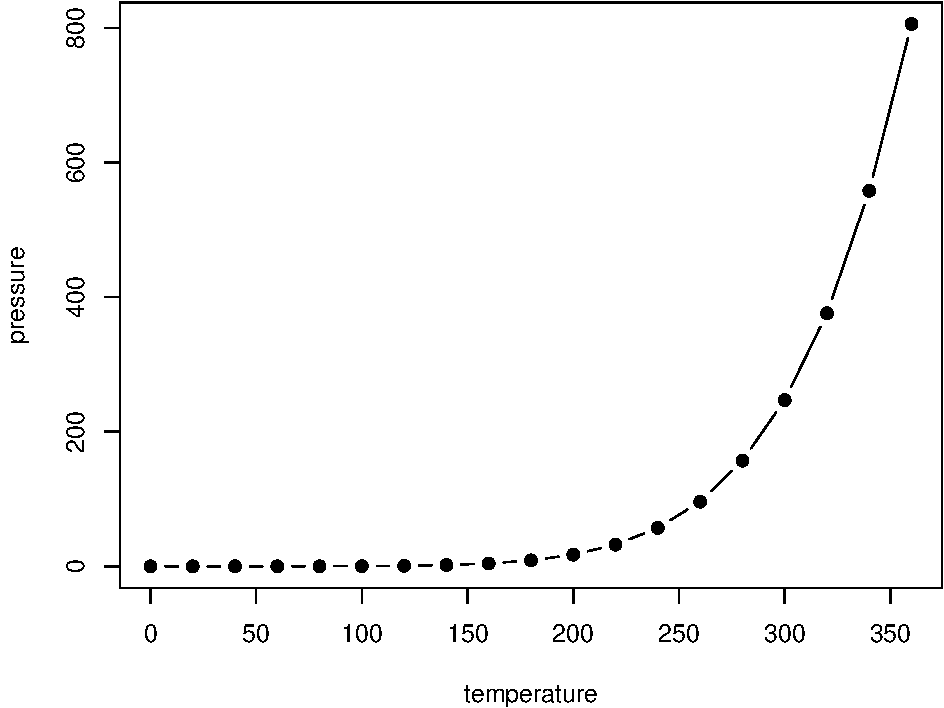
\includegraphics[width=0.8\linewidth]{group1_BenediktKronhardt_BorgeMeyer_files/figure-latex/nice-fig-1} 

}

\caption{Here is a nice figure!}\label{fig:nice-fig}
\end{figure}

Don't miss Table \ref{tab:nice-tab}.

\linespread{1}

\begin{Shaded}
\begin{Highlighting}[]
\NormalTok{knitr}\SpecialCharTok{::}\FunctionTok{kable}\NormalTok{(}
  \FunctionTok{head}\NormalTok{(pressure, }\DecValTok{10}\NormalTok{), }\AttributeTok{caption =} \StringTok{\textquotesingle{}Here is a nice table!\textquotesingle{}}\NormalTok{,}
  \AttributeTok{booktabs =} \ConstantTok{TRUE}
\NormalTok{)}
\end{Highlighting}
\end{Shaded}

\linespread{1}

\begin{table}

\caption{\label{tab:nice-tab}Here is a nice table!}
\centering
\begin{tabular}[t]{rr}
\toprule
temperature & pressure\\
\midrule
0 & 0.0002\\
20 & 0.0012\\
40 & 0.0060\\
60 & 0.0300\\
80 & 0.0900\\
\addlinespace
100 & 0.2700\\
120 & 0.7500\\
140 & 1.8500\\
160 & 4.2000\\
180 & 8.8000\\
\bottomrule
\end{tabular}
\end{table}

\hypertarget{parts}{%
\chapter{Parts}\label{parts}}

You can add parts to organize one or more book chapters together. Parts can be inserted at the top of an .Rmd file, before the first-level chapter heading in that same file.

Add a numbered part: \texttt{\#\ (PART)\ Act\ one\ \{-\}} (followed by \texttt{\#\ A\ chapter})

Add an unnumbered part: \texttt{\#\ (PART\textbackslash{}*)\ Act\ one\ \{-\}} (followed by \texttt{\#\ A\ chapter})

Add an appendix as a special kind of un-numbered part: \texttt{\#\ (APPENDIX)\ Other\ stuff\ \{-\}} (followed by \texttt{\#\ A\ chapter}). Chapters in an appendix are prepended with letters instead of numbers.

\hypertarget{footnotes-and-citations}{%
\chapter{Footnotes and citations}\label{footnotes-and-citations}}

\hypertarget{footnotes}{%
\section{Footnotes}\label{footnotes}}

Footnotes are put inside the square brackets after a caret \texttt{\^{}{[}{]}}. Like this one \footnote{This is a footnote.}.

\hypertarget{citations}{%
\section{Citations}\label{citations}}

Reference items in your bibliography file(s) using \texttt{@key}.

For example, we are using the \textbf{bookdown} package (\protect\hyperlink{ref-R-bookdown}{Xie 2022}) (check out the last code chunk in index.Rmd to see how this citation key was added) in this sample book, which was built on top of R Markdown and \textbf{knitr} (\protect\hyperlink{ref-xie2015}{Xie 2015}) (this citation was added manually in an external file book.bib).
Note that the \texttt{.bib} files need to be listed in the index.Rmd with the YAML \texttt{bibliography} key.

The RStudio Visual Markdown Editor can also make it easier to insert citations: \url{https://rstudio.github.io/visual-markdown-editing/\#/citations}

\hypertarget{blocks}{%
\chapter{Blocks}\label{blocks}}

\hypertarget{equations}{%
\section{Equations}\label{equations}}

Here is an equation.

\begin{equation} 
  f\left(k\right) = \binom{n}{k} p^k\left(1-p\right)^{n-k}
  \label{eq:binom}
\end{equation}

You may refer to using \texttt{\textbackslash{}@ref(eq:binom)}, like see Equation \eqref{eq:binom}.

\hypertarget{theorems-and-proofs}{%
\section{Theorems and proofs}\label{theorems-and-proofs}}

Labeled theorems can be referenced in text using \texttt{\textbackslash{}@ref(thm:tri)}, for example, check out this smart theorem \ref{thm:tri}.

\begin{theorem}
\protect\hypertarget{thm:tri}{}\label{thm:tri}For a right triangle, if \(c\) denotes the \emph{length} of the hypotenuse
and \(a\) and \(b\) denote the lengths of the \textbf{other} two sides, we have
\[a^2 + b^2 = c^2\]
\end{theorem}

Read more here \url{https://bookdown.org/yihui/bookdown/markdown-extensions-by-bookdown.html}.

\hypertarget{callout-blocks}{%
\section{Callout blocks}\label{callout-blocks}}

The R Markdown Cookbook provides more help on how to use custom blocks to design your own callouts: \url{https://bookdown.org/yihui/rmarkdown-cookbook/custom-blocks.html}

\hypertarget{sharing-your-book}{%
\chapter{Sharing your book}\label{sharing-your-book}}

\hypertarget{publishing}{%
\section{Publishing}\label{publishing}}

HTML books can be published online, see: \url{https://bookdown.org/yihui/bookdown/publishing.html}

\hypertarget{pages}{%
\section{404 pages}\label{pages}}

By default, users will be directed to a 404 page if they try to access a webpage that cannot be found. If you'd like to customize your 404 page instead of using the default, you may add either a \texttt{\_404.Rmd} or \texttt{\_404.md} file to your project root and use code and/or Markdown syntax.

\hypertarget{metadata-for-sharing}{%
\section{Metadata for sharing}\label{metadata-for-sharing}}

Bookdown HTML books will provide HTML metadata for social sharing on platforms like Twitter, Facebook, and LinkedIn, using information you provide in the \texttt{index.Rmd} YAML. To setup, set the \texttt{url} for your book and the path to your \texttt{cover-image} file. Your book's \texttt{title} and \texttt{description} are also used.

This \texttt{gitbook} uses the same social sharing data across all chapters in your book- all links shared will look the same.

Specify your book's source repository on GitHub using the \texttt{edit} key under the configuration options in the \texttt{\_output.yml} file, which allows users to suggest an edit by linking to a chapter's source file.

Read more about the features of this output format here:

\url{https://pkgs.rstudio.com/bookdown/reference/gitbook.html}

Or use:

\linespread{1}

\begin{Shaded}
\begin{Highlighting}[]
\NormalTok{?bookdown}\SpecialCharTok{::}\NormalTok{gitbook}
\end{Highlighting}
\end{Shaded}

\linespread{1}

\pagebreak

\hypertarget{references}{%
\chapter*{References}\label{references}}
\addcontentsline{toc}{chapter}{References}

\hypertarget{refs}{}
\begin{CSLReferences}{1}{0}
\leavevmode\vadjust pre{\hypertarget{ref-R-rmarkdown}{}}%
Allaire, JJ, Yihui Xie, Jonathan McPherson, Javier Luraschi, Kevin Ushey, Aron Atkins, Hadley Wickham, Joe Cheng, Winston Chang, and Richard Iannone. 2022. \emph{Rmarkdown: Dynamic Documents for r}. \url{https://CRAN.R-project.org/package=rmarkdown}.

\leavevmode\vadjust pre{\hypertarget{ref-dawson1995}{}}%
Dawson, Robert J. MacG. 1995. {``The "Unusual Episode" Data Revisited.''} \emph{Journal of Statistics Education} 3 (3): 1--9. \url{https://doi.org/10.1080/10691898.1995.11910499}.

\leavevmode\vadjust pre{\hypertarget{ref-fox2003}{}}%
Fox, John. 2003. {``Effect Displays in {R} for Generalised Linear Models.''} \emph{Journal of Statistical Software} 8 (15): 1--27. \url{https://doi.org/10.18637/jss.v008.i15}.

\leavevmode\vadjust pre{\hypertarget{ref-fox2019}{}}%
Fox, John, and Sanford Weisberg. 2019. \emph{An {R} Companion to Applied Regression}. 3rd ed. Thousand Oaks {CA}: Sage. \url{https://socialsciences.mcmaster.ca/jfox/Books/Companion/}.

\leavevmode\vadjust pre{\hypertarget{ref-Hmisc2022}{}}%
Harrell Jr, Frank E. 2022. \emph{Hmisc: {Harrell Miscellaneous}}. \url{https://CRAN.R-project.org/package=Hmisc}.

\leavevmode\vadjust pre{\hypertarget{ref-harrell2019}{}}%
Harrell, Jr., Frank E. 2019. \emph{Regression Modeling Strategies}. 2nd ed. Switzerland: Springer Cham. \url{https://hbiostat.org/doc/rms/}.

\leavevmode\vadjust pre{\hypertarget{ref-Lenth2022}{}}%
Lenth, Russell V. 2022. \emph{Emmeans: {Estimated Marginal Means, aka Least-Squares Means}}. \url{https://CRAN.R-project.org/package=emmeans}.

\leavevmode\vadjust pre{\hypertarget{ref-jtools}{}}%
Long, Jacob A. 2022. \emph{Jtools: {Analysis and Presentation of Social Scientific Data}}. \url{https://cran.r-project.org/package=jtools}.

\leavevmode\vadjust pre{\hypertarget{ref-Luedecke2018}{}}%
Lüdecke, Daniel. 2018. {``Ggeffects: {Tidy Data Frames of Marginal Effects from Regression Models}.''} \emph{Journal of Open Source Software} 3 (26): 772. \url{https://doi.org/10.21105/joss.00772}.

\leavevmode\vadjust pre{\hypertarget{ref-Luedecke-see2021}{}}%
Lüdecke, Daniel, Indrajeet Patil, Mattan S. Ben-Shachar, Brenton M. Wiernik, Philip Waggoner, and Dominique Makowski. 2021. {``{see}: An {R} Package for Visualizing Statistical Models.''} \emph{Journal of Open Source Software} 6 (64): 3393. \url{https://doi.org/10.21105/joss.03393}.

\leavevmode\vadjust pre{\hypertarget{ref-Makowski2021}{}}%
Makowski, Dominique, Mattan S. Ben-Shachar, Indrajeet Patil, and Daniel Lüdecke. 2021. {``Automated Results Reporting as a Practical Tool to Improve Reproducibility and Methodological Best Practices Adoption.''} \emph{CRAN}. \url{https://github.com/easystats/report}.

\leavevmode\vadjust pre{\hypertarget{ref-nelder1972}{}}%
Nelder, John A., and Robert W. M. Wedderburn. 1972. {``Generalized Linear Models.''} \emph{{Journal of the Royal Statistical Society. Series A (General)}} 135 (3): 370--84. \url{http://www.jstor.org/stable/2344614}.

\leavevmode\vadjust pre{\hypertarget{ref-Pedersen2022}{}}%
Pedersen, Thomas Lin. 2022. \emph{Patchwork: The Composer of Plots}. \url{https://CRAN.R-project.org/package=patchwork}.

\leavevmode\vadjust pre{\hypertarget{ref-R-base}{}}%
R Core Team. 2022. \emph{R: A Language and Environment for Statistical Computing}. Vienna, Austria: R Foundation for Statistical Computing. \url{https://www.R-project.org/}.

\leavevmode\vadjust pre{\hypertarget{ref-introR2022}{}}%
Venables, W. N., D. M. Smith, and the R Core Team. 2022. \emph{{An Introduction to R}}. Version 4.2.1. Vienna, Austria: R Foundation for Statistical Computing. \url{https://cran.r-project.org/doc/manuals/r-release/R-intro.html}.

\leavevmode\vadjust pre{\hypertarget{ref-xie2015}{}}%
Xie, Yihui. 2015. \emph{Dynamic Documents with {R} and Knitr}. 2nd ed. Boca Raton, Florida: Chapman; Hall/CRC. \url{http://yihui.org/knitr/}.

\leavevmode\vadjust pre{\hypertarget{ref-R-bookdown}{}}%
---------. 2022. \emph{Bookdown: Authoring Books and Technical Documents with r Markdown}. \url{https://CRAN.R-project.org/package=bookdown}.

\end{CSLReferences}

\newpage

\hypertarget{declaration-of-honor}{%
\chapter*{Declaration of Honor}\label{declaration-of-honor}}
\addcontentsline{toc}{chapter}{Declaration of Honor}

We hereby declare that

\begin{enumerate}
\def\labelenumi{\arabic{enumi}.}
\tightlist
\item
  we wrote this project report without the assistance of others;
\item
  we have marked direct quotes used from the literature and the use of ideas of other authors at the corresponding locations in the thesis;
\item
  we have not presented this thesis for any other exam. We acknowledge that a false declaration will have legal consequences.
\end{enumerate}

Hamburg, dd.mm.yyyy

aaaaa, bbbbbb

\vspace{2.5cm}

We accept that the HSBA may check the originality of our work using a range of manual and computer based techniques, including transferring and storing our submission in a database for the purpose of data-matching to help detect plagiarism.

Hamburg, dd.mm.yyyy

aaaaa, bbbbbb

\hypertarget{appendix-appendix}{%
\appendix}


\hypertarget{useful-code-examples}{%
\chapter{Useful code examples}\label{useful-code-examples}}

\hypertarget{use-of-acronyms}{%
\section{Use of acronyms}\label{use-of-acronyms}}

To begin, let's see how the list of acronyms is working. The acronyms are defined in the file \texttt{abbreviations.tex}, see an explanation of how to do that in the file itself. Regarding the use of these acronyms inside of the text: In the source code, one writes something as follows, using standard \LaTeX~commands:

\begin{verbatim}
First use: \Ac{cran}. Second use: \ac{cran}. First use of another abbreviation: 
\ac{ide}, then the plural use: \acp{ide}. And here you see that \acs{H2O} 
is actually \ac{H2O}.
\end{verbatim}

This displays as follows:

\begin{quote}
First use: \Ac{cran}. Second use: \ac{cran}.
First use of another abbreviation: \ac{ide}, then the plural use: \acp{ide}.
And here you see that \acs{H2O} is actually \ac{H2O}.
\end{quote}

\hypertarget{read-data}{%
\section{Load packages and read data into R}\label{read-data}}

At the beginning of your book, you should put all necessary packages in one chunk, then loading the data in the next chunk so that these steps are properly organized:

\linespread{1}

\begin{Shaded}
\begin{Highlighting}[]
\FunctionTok{library}\NormalTok{(tidyverse) }\CommentTok{\# This includes readr!}
\FunctionTok{library}\NormalTok{(xtable) }\CommentTok{\# For displaying LaTeX tables}
\FunctionTok{library}\NormalTok{(modelsummary) }\CommentTok{\# For displaying regression models in tables}
\FunctionTok{library}\NormalTok{(stargazer) }\CommentTok{\# For displaying regression models in tables}
\FunctionTok{library}\NormalTok{(jtools) }\CommentTok{\# For displaying regression models in tables}
\FunctionTok{library}\NormalTok{(kableExtra) }\CommentTok{\# For displaying or changing tables}
\FunctionTok{library}\NormalTok{(gt) }\CommentTok{\# For displaying tables}
\FunctionTok{library}\NormalTok{(gtsummary) }\CommentTok{\# For model reporting inline and in tables}
\FunctionTok{library}\NormalTok{(broom) }\CommentTok{\# For working with statistical models}
\FunctionTok{library}\NormalTok{(car) }\CommentTok{\# For type{-}III anova tests}
\FunctionTok{library}\NormalTok{(report) }\CommentTok{\# For automated text{-}based model reporting}
\FunctionTok{library}\NormalTok{(effects) }\CommentTok{\# For working with statistical models / visualize effects}
\FunctionTok{library}\NormalTok{(ggeffects) }\CommentTok{\# For working with statistical models / visualize effects}
\FunctionTok{library}\NormalTok{(patchwork) }\CommentTok{\# For putting different visualizations in one figure}
\end{Highlighting}
\end{Shaded}

\linespread{1}

One of the most common ways to get your data into R is to place them into your project directory as a CSV-file and read them into the current session, that is, the session of the produced book, using \href{https://cran.r-project.org/web/packages/readr/}{readr} (\url{https://cran.r-project.org/web/packages/readr/}).

\linespread{1}

\begin{Shaded}
\begin{Highlighting}[]
\NormalTok{df1 }\OtherTok{\textless{}{-}} \FunctionTok{read\_csv}\NormalTok{(}\StringTok{"02{-}data/mpg\_data\_as\_csv.csv"}\NormalTok{, }\AttributeTok{lazy =} \ConstantTok{FALSE}\NormalTok{)}
\end{Highlighting}
\end{Shaded}

\linespread{1}

\begin{verbatim}
#> Rows: 234 Columns: 11
#> -- Column specification ------------------
#> Delimiter: ","
#> chr (6): manufacturer, model, trans, drv, fl, class
#> dbl (5): displ, year, cyl, cty, hwy
#> 
#> i Use `spec()` to retrieve the full column specification for this data.
#> i Specify the column types or set `show_col_types = FALSE` to quiet this message.
\end{verbatim}

You can then use the function arguments to change necessary things like the delimiter (also switching to \texttt{readr::read\_delim()} instead of \texttt{readr::read\_csv()} to do this), or see the specifics of the column types using \texttt{read::spec()} and change them accordingly if needed.

\linespread{1}

\begin{Shaded}
\begin{Highlighting}[]
\FunctionTok{spec}\NormalTok{(df1)}
\end{Highlighting}
\end{Shaded}

\linespread{1}

\begin{verbatim}
#> cols(
#>   manufacturer = col_character(),
#>   model = col_character(),
#>   displ = col_double(),
#>   year = col_double(),
#>   cyl = col_double(),
#>   trans = col_character(),
#>   drv = col_character(),
#>   cty = col_double(),
#>   hwy = col_double(),
#>   fl = col_character(),
#>   class = col_character()
#> )
\end{verbatim}

\linespread{1}

\begin{Shaded}
\begin{Highlighting}[]

\NormalTok{df1 }\OtherTok{\textless{}{-}} \FunctionTok{read\_delim}\NormalTok{(}\StringTok{"02{-}data/mpg\_data\_as\_csv.csv"}\NormalTok{,}
                  \AttributeTok{delim =} \StringTok{","}\NormalTok{,}
                  \AttributeTok{col\_types =} \FunctionTok{cols}\NormalTok{(}
                      \AttributeTok{manufacturer =} \FunctionTok{col\_character}\NormalTok{(),}
                      \AttributeTok{model =} \FunctionTok{col\_character}\NormalTok{(),}
                      \AttributeTok{displ =} \FunctionTok{col\_double}\NormalTok{(),}
                      \AttributeTok{year =} \FunctionTok{col\_double}\NormalTok{(),}
                      \AttributeTok{cyl =} \FunctionTok{col\_double}\NormalTok{(),}
                      \AttributeTok{trans =} \FunctionTok{col\_character}\NormalTok{(),}
                      \AttributeTok{drv =} \FunctionTok{col\_character}\NormalTok{(),}
                      \AttributeTok{cty =} \FunctionTok{col\_double}\NormalTok{(),}
                      \AttributeTok{hwy =} \FunctionTok{col\_double}\NormalTok{(),}
                      \AttributeTok{fl =} \FunctionTok{col\_character}\NormalTok{(),}
                      \AttributeTok{class =} \FunctionTok{col\_character}\NormalTok{()}
\NormalTok{                      ), }\AttributeTok{lazy =} \ConstantTok{FALSE}
\NormalTok{                  )}
\end{Highlighting}
\end{Shaded}

\linespread{1}

\hypertarget{displaying-different-types-of-tables-from-modelsummary}{%
\section{Displaying different types of tables from modelsummary}\label{displaying-different-types-of-tables-from-modelsummary}}

The data set is part of the \href{https://cran.r-project.org/web/packages/ggplot2/}{ggplot2} package (\url{https://cran.r-project.org/web/packages/ggplot2/}) and is originally named \texttt{mpg}. To display a summary of the data set in your work, you may use, for example, the modelsummary package with its function \texttt{modelsummary::datasummary\_skim()}, from which the output can be seen in table \ref{tab:skim-df1}. Don't forget to name the chunk and specify the table caption using the argument \texttt{title} in the function call! Without these two adjustments, you cannot cross-reference this table and it does not appear in the list of tables in the frontmatter. Another source of error is the naming of the chunks: Never use underscores in these, only letters and minus signs! And always place a blank line in front and after a code chunk.

\linespread{1}

\begin{Shaded}
\begin{Highlighting}[]
\CommentTok{\# You can reference this table now with "\textbackslash{}@ref(tab:skim{-}df1)".}
\CommentTok{\# The part with kable\_styling is coming from the kableExtra package and }
\CommentTok{\# changes the position of the table and its appearance}
\FunctionTok{datasummary\_skim}\NormalTok{(df1, }\AttributeTok{output =} \StringTok{\textquotesingle{}kableExtra\textquotesingle{}}\NormalTok{, }\AttributeTok{booktabs =} \ConstantTok{TRUE}\NormalTok{,}
        \AttributeTok{title =} \StringTok{"Overview of the numerical variables in data set df1"}\NormalTok{) }\SpecialCharTok{\%\textgreater{}\%}
    \FunctionTok{kable\_styling}\NormalTok{(}\AttributeTok{latex\_options =} \FunctionTok{c}\NormalTok{(}\StringTok{"striped"}\NormalTok{, }\StringTok{"HOLD\_position"}\NormalTok{))}
\end{Highlighting}
\end{Shaded}

\linespread{1}

\begin{table}[H]

\caption{\label{tab:skim-df1}Overview of the numerical variables in data set df1}
\centering
\begin{tabular}[t]{lrrrrrrr>{}r}
\toprule
  & Unique (\#) & Missing (\%) & Mean & SD & Min & Median & Max &   \\
\midrule
\cellcolor{gray!6}{displ} & \cellcolor{gray!6}{35} & \cellcolor{gray!6}{0} & \cellcolor{gray!6}{\num{3.5}} & \cellcolor{gray!6}{\num{1.3}} & \cellcolor{gray!6}{\num{1.6}} & \cellcolor{gray!6}{\num{3.3}} & \cellcolor{gray!6}{\num{7.0}} & \cellcolor{gray!6}{
\includegraphics[width=0.67in, height=0.17in]{C:/Users/kronh/OneDrive/Dokumente/R_Projects/group1_BenediktKronhardt_BorgeMeyer/group1_BenediktKronhardt_BorgeMeyer_files/figure-latex/hist_542c2df2a08.pdf}}\\
year & 2 & 0 & \num{2003.5} & \num{4.5} & \num{1999.0} & \num{2003.5} & \num{2008.0} & 
\includegraphics[width=0.67in, height=0.17in]{C:/Users/kronh/OneDrive/Dokumente/R_Projects/group1_BenediktKronhardt_BorgeMeyer/group1_BenediktKronhardt_BorgeMeyer_files/figure-latex/hist_542c638bd3b.pdf}\\
\cellcolor{gray!6}{cyl} & \cellcolor{gray!6}{4} & \cellcolor{gray!6}{0} & \cellcolor{gray!6}{\num{5.9}} & \cellcolor{gray!6}{\num{1.6}} & \cellcolor{gray!6}{\num{4.0}} & \cellcolor{gray!6}{\num{6.0}} & \cellcolor{gray!6}{\num{8.0}} & \cellcolor{gray!6}{
\includegraphics[width=0.67in, height=0.17in]{C:/Users/kronh/OneDrive/Dokumente/R_Projects/group1_BenediktKronhardt_BorgeMeyer/group1_BenediktKronhardt_BorgeMeyer_files/figure-latex/hist_542c5afc1934.pdf}}\\
cty & 21 & 0 & \num{16.9} & \num{4.3} & \num{9.0} & \num{17.0} & \num{35.0} & 
\includegraphics[width=0.67in, height=0.17in]{C:/Users/kronh/OneDrive/Dokumente/R_Projects/group1_BenediktKronhardt_BorgeMeyer/group1_BenediktKronhardt_BorgeMeyer_files/figure-latex/hist_542c7893135.pdf}\\
\cellcolor{gray!6}{hwy} & \cellcolor{gray!6}{27} & \cellcolor{gray!6}{0} & \cellcolor{gray!6}{\num{23.4}} & \cellcolor{gray!6}{\num{6.0}} & \cellcolor{gray!6}{\num{12.0}} & \cellcolor{gray!6}{\num{24.0}} & \cellcolor{gray!6}{\num{44.0}} & \cellcolor{gray!6}{
\includegraphics[width=0.67in, height=0.17in]{C:/Users/kronh/OneDrive/Dokumente/R_Projects/group1_BenediktKronhardt_BorgeMeyer/group1_BenediktKronhardt_BorgeMeyer_files/figure-latex/hist_542c5a16dd3.pdf}}\\
\bottomrule
\end{tabular}
\end{table}

Another useful table can be produced by using the function \texttt{datasummary\_correlation()} from the same package. Its output can be seen in table \ref{tab:corr-df1}, which in addition is changed to show how to use footnotes using \texttt{kableExtra}. The content of the footnote is also true for table \ref{tab:skim-df1}, so be careful and adjust variable types before doing something with them such as in table \ref{tab:skim-df1-cat}.

\linespread{1}

\begin{Shaded}
\begin{Highlighting}[]
\NormalTok{df1\_footnote }\OtherTok{\textless{}{-}}\NormalTok{ df1}
\FunctionTok{names}\NormalTok{(df1\_footnote)[}\FunctionTok{names}\NormalTok{(df1\_footnote) }\SpecialCharTok{==} \StringTok{"year"}\NormalTok{] }\OtherTok{\textless{}{-}} 
    \FunctionTok{paste0}\NormalTok{(}\FunctionTok{names}\NormalTok{(df1\_footnote)[}\FunctionTok{names}\NormalTok{(df1\_footnote) }\SpecialCharTok{==} \StringTok{"year"}\NormalTok{], }
           \FunctionTok{footnote\_marker\_symbol}\NormalTok{(}\DecValTok{1}\NormalTok{, }\StringTok{"latex"}\NormalTok{))}

\FunctionTok{datasummary\_correlation}\NormalTok{(df1\_footnote, }\AttributeTok{output =} \StringTok{\textquotesingle{}kableExtra\textquotesingle{}}\NormalTok{,}
        \AttributeTok{booktabs =} \ConstantTok{TRUE}\NormalTok{, }\AttributeTok{escape =} \ConstantTok{FALSE}\NormalTok{, }\CommentTok{\# \textquotesingle{}escape = FALSE\textquotesingle{} here is important!}
        \AttributeTok{title =} \StringTok{"Correlations of numerical variables in data set df1"}\NormalTok{) }\SpecialCharTok{\%\textgreater{}\%} 
    \FunctionTok{kable\_styling}\NormalTok{(}\AttributeTok{latex\_options =} \FunctionTok{c}\NormalTok{(}\StringTok{"striped"}\NormalTok{, }\StringTok{"HOLD\_position"}\NormalTok{)) }\SpecialCharTok{\%\textgreater{}\%} 
    \FunctionTok{footnote}\NormalTok{(}\AttributeTok{symbol =} \FunctionTok{paste0}\NormalTok{(}\StringTok{"Using the categorical variable"}\NormalTok{,}
                             \StringTok{" \textquotesingle{}year\textquotesingle{} here in a correlation is :{-}("}\NormalTok{),}
             \AttributeTok{threeparttable =} \ConstantTok{TRUE}\NormalTok{) }\CommentTok{\# This last options enables the line break!}
\end{Highlighting}
\end{Shaded}

\linespread{1}

\begin{table}[H]

\caption{\label{tab:corr-df1}Correlations of numerical variables in data set df1}
\centering
\begin{threeparttable}
\begin{tabular}[t]{lrrrrr}
\toprule
  & displ & year\textsuperscript{*} & cyl & cty & hwy\\
\midrule
\cellcolor{gray!6}{displ} & \cellcolor{gray!6}{1} & \cellcolor{gray!6}{.} & \cellcolor{gray!6}{.} & \cellcolor{gray!6}{.} & \cellcolor{gray!6}{.}\\
year\textsuperscript{*} & \num{.15} & 1 & . & . & .\\
\cellcolor{gray!6}{cyl} & \cellcolor{gray!6}{\num{.93}} & \cellcolor{gray!6}{\num{.12}} & \cellcolor{gray!6}{1} & \cellcolor{gray!6}{.} & \cellcolor{gray!6}{.}\\
cty & \num{-.80} & \num{-.04} & \num{-.81} & 1 & .\\
\cellcolor{gray!6}{hwy} & \cellcolor{gray!6}{\num{-.77}} & \cellcolor{gray!6}{\num{.00}} & \cellcolor{gray!6}{\num{-.76}} & \cellcolor{gray!6}{\num{.96}} & \cellcolor{gray!6}{1}\\
\bottomrule
\end{tabular}
\begin{tablenotes}
\item[*] Using the categorical variable 'year' here in a correlation is :-(
\end{tablenotes}
\end{threeparttable}
\end{table}

Adjusting all categorical variables to the correct type:

\linespread{1}

\begin{Shaded}
\begin{Highlighting}[]
\NormalTok{df1 }\OtherTok{\textless{}{-}}\NormalTok{ df1 }\SpecialCharTok{\%\textgreater{}\%} 
    \FunctionTok{mutate}\NormalTok{(}\AttributeTok{manufacturer =} \FunctionTok{factor}\NormalTok{(manufacturer),}
           \AttributeTok{model =} \FunctionTok{factor}\NormalTok{(model),}
           \AttributeTok{year =} \FunctionTok{factor}\NormalTok{(year),}
           \AttributeTok{cyl =} \FunctionTok{ordered}\NormalTok{(cyl, }
                         \AttributeTok{levels =} \FunctionTok{c}\NormalTok{(}\DecValTok{4}\NormalTok{,}\DecValTok{5}\NormalTok{,}\DecValTok{6}\NormalTok{,}\DecValTok{8}\NormalTok{),}
                         \AttributeTok{labels =} \FunctionTok{c}\NormalTok{(}\StringTok{"4 Cylinders"}\NormalTok{,}
                                    \StringTok{"5 Cylinders"}\NormalTok{,}
                                    \StringTok{"6 Cylinders"}\NormalTok{,}
                                    \StringTok{"8 Cylinders"}\NormalTok{)),}
           \AttributeTok{trans =} \FunctionTok{factor}\NormalTok{(trans),}
           \AttributeTok{drv =} \FunctionTok{factor}\NormalTok{(drv, }
                        \AttributeTok{levels =} \FunctionTok{c}\NormalTok{(}\StringTok{"f"}\NormalTok{, }\StringTok{"r"}\NormalTok{, }\StringTok{"4"}\NormalTok{),}
                        \AttributeTok{labels =} \FunctionTok{c}\NormalTok{(}\StringTok{"Front wheel drive"}\NormalTok{,}
                                   \StringTok{"Rear wheel drive"}\NormalTok{,}
                                   \StringTok{"4 wheel drive"}\NormalTok{)),}
           \AttributeTok{fl =} \FunctionTok{factor}\NormalTok{(fl),}
           \AttributeTok{class =} \FunctionTok{factor}\NormalTok{(class)) }
\end{Highlighting}
\end{Shaded}

\linespread{1}

Now using another kind of table from the \texttt{modelsummary} package:

\linespread{1}

\begin{Shaded}
\begin{Highlighting}[]
\FunctionTok{datasummary\_crosstab}\NormalTok{(drv }\SpecialCharTok{\textasciitilde{}}\NormalTok{ year, }
                     \AttributeTok{data =}\NormalTok{ df1, }\AttributeTok{booktabs =} \ConstantTok{TRUE}\NormalTok{,}
        \AttributeTok{title =} \StringTok{"Cross tabulations for year and type of drive"}\NormalTok{) }\SpecialCharTok{\%\textgreater{}\%} 
    \FunctionTok{kable\_styling}\NormalTok{(}\AttributeTok{latex\_options =} \FunctionTok{c}\NormalTok{(}\StringTok{"striped"}\NormalTok{, }\StringTok{"HOLD\_position"}\NormalTok{))}
\end{Highlighting}
\end{Shaded}

\linespread{1}

\begin{table}[H]

\caption{\label{tab:skim-df1-cat}Cross tabulations for year and type of drive}
\centering
\begin{tabular}[t]{llrrr}
\toprule
drv &   & 1999 & 2008 & All\\
\midrule
\cellcolor{gray!6}{Front wheel drive} & \cellcolor{gray!6}{N} & \cellcolor{gray!6}{57} & \cellcolor{gray!6}{49} & \cellcolor{gray!6}{106}\\
 & \% row & \num{53.8} & \num{46.2} & \num{100.0}\\
\cellcolor{gray!6}{Rear wheel drive} & \cellcolor{gray!6}{N} & \cellcolor{gray!6}{11} & \cellcolor{gray!6}{14} & \cellcolor{gray!6}{25}\\
 & \% row & \num{44.0} & \num{56.0} & \num{100.0}\\
\cellcolor{gray!6}{4 wheel drive} & \cellcolor{gray!6}{N} & \cellcolor{gray!6}{49} & \cellcolor{gray!6}{54} & \cellcolor{gray!6}{103}\\
 & \% row & \num{47.6} & \num{52.4} & \num{100.0}\\
\cellcolor{gray!6}{All} & \cellcolor{gray!6}{N} & \cellcolor{gray!6}{117} & \cellcolor{gray!6}{117} & \cellcolor{gray!6}{234}\\
 & \% row & \num{50.0} & \num{50.0} & \num{100.0}\\
\bottomrule
\end{tabular}
\end{table}

See the \texttt{datasummary} vignettes for more possibilities:

\begin{quote}
\url{https://vincentarelbundock.github.io/modelsummary/articles/datasummary.html}
\end{quote}

\hypertarget{reporting-statistical-models}{%
\section{Reporting statistical models}\label{reporting-statistical-models}}

\hypertarget{t-test}{%
\subsection{\texorpdfstring{\(t\)-test}{t-test}}\label{t-test}}

In the following paragraphs, I want to give some examples on how to report a statistical model. Let's start with a simple one, an independent two sample \(t\)-test:

\begin{equation} 
  t = \frac{m_A - m_B}{\sqrt{ \frac{s^2}{n_A} + \frac{s^2}{n_B} }}
  \label{eq:t-test}
\end{equation}

where \(s^2\) is an estimator of the common variance of the two samples. It can be calculated as

\begin{equation} 
  s^2 = \frac{\sum{(x-m_A)^2}+\sum{(x-m_B)^2}}{n_A+n_B-2}
  \label{eq:t-test-s}
\end{equation}

Once the \(t\)-test statistic value is calculated, one uses the critical value of Student's \(t\)-distribution corresponding to the significance level alpha of your choice (5\%). The degrees of freedom (\(df\)) used in this test are \(df = n_A + n_B - 2\). We can simulate some data according to equation \eqref{eq:t-test} and apply the function \texttt{t.test()} from the \texttt{stats} package:

\linespread{1}

\begin{Shaded}
\begin{Highlighting}[]
\NormalTok{N }\OtherTok{\textless{}{-}} \DecValTok{100}
\NormalTok{delta }\OtherTok{\textless{}{-}} \DecValTok{5}
\NormalTok{same\_sd }\OtherTok{\textless{}{-}} \DecValTok{5}
\NormalTok{df\_ttest }\OtherTok{\textless{}{-}} \FunctionTok{tibble}\NormalTok{(}\AttributeTok{class =} \FunctionTok{gl}\NormalTok{(}\AttributeTok{n =} \DecValTok{2}\NormalTok{, }\AttributeTok{k =}\NormalTok{ N}\SpecialCharTok{/}\DecValTok{2}\NormalTok{, }\AttributeTok{labels =} \FunctionTok{c}\NormalTok{(}\StringTok{"Class A"}\NormalTok{, }\StringTok{"Class B"}\NormalTok{)),}
                   \AttributeTok{exam\_score =} \FunctionTok{c}\NormalTok{(}\FunctionTok{rnorm}\NormalTok{(N}\SpecialCharTok{/}\DecValTok{2}\NormalTok{, }\AttributeTok{mean =} \DecValTok{50}\NormalTok{, }\AttributeTok{sd =}\NormalTok{ same\_sd),}
                                  \FunctionTok{rnorm}\NormalTok{(N}\SpecialCharTok{/}\DecValTok{2}\NormalTok{, }\AttributeTok{mean =} \DecValTok{50} \SpecialCharTok{+}\NormalTok{ delta, }\AttributeTok{sd =}\NormalTok{ same\_sd)))}
\NormalTok{test1 }\OtherTok{\textless{}{-}} \FunctionTok{t.test}\NormalTok{(exam\_score }\SpecialCharTok{\textasciitilde{}}\NormalTok{ class, }\AttributeTok{data =}\NormalTok{ df\_ttest, }\AttributeTok{var.equal =} \ConstantTok{TRUE}\NormalTok{)}
\NormalTok{test1\_glance }\OtherTok{\textless{}{-}} \FunctionTok{glance}\NormalTok{(test1)}
\NormalTok{test1}
\end{Highlighting}
\end{Shaded}

\linespread{1}

\begin{verbatim}
#> 
#>  Two Sample t-test
#> 
#> data:  exam_score by class
#> t = -3.3958, df = 98, p-value = 0.0009897
#> alternative hypothesis: true difference in means between group Class A and group Class B is not equal to 0
#> 95 percent confidence interval:
#>  -5.811927 -1.524531
#> sample estimates:
#> mean in group Class A mean in group Class B 
#>              50.24124              53.90946
\end{verbatim}

This console output is not very pleasant and should not be reported as this. Better to use the package \texttt{broom} and its function \texttt{broom::glance()} to extract everything you need using inline code chunks, which gives you a significant difference of \(\approx~-3.67\) between class A (\(M = 50.24\), \(SD = 5.67\)) and class B (\(M = 53.91\), \(SD = 5.11\)) in this case, \(t(98)~=~-3.396,~p~=~0.001\). You should read the source code of this paragraph carefully to see how everything in the inline chunks fits together to produce such an output.

\hypertarget{chi2-test}{%
\subsection{\texorpdfstring{\(\chi^2\)-test}{\textbackslash chi\^{}2-test}}\label{chi2-test}}

The same procedure can be used to report a \(\chi^2\)-test using the function \texttt{chisq.test()} from the \texttt{stats} package. This time, let's use the \texttt{mpg} data set imported above in section \ref{read-data}:

\linespread{1}

\begin{Shaded}
\begin{Highlighting}[]
\CommentTok{\# Build a contingency table for year and cylinders}
\NormalTok{tbl\_df }\OtherTok{\textless{}{-}} \FunctionTok{table}\NormalTok{(df1}\SpecialCharTok{$}\NormalTok{year, df1}\SpecialCharTok{$}\NormalTok{cyl)}
\NormalTok{chi\_test }\OtherTok{\textless{}{-}} \FunctionTok{chisq.test}\NormalTok{(tbl\_df)}
\NormalTok{chi\_result }\OtherTok{\textless{}{-}} \FunctionTok{glance}\NormalTok{(chi\_test)}
\NormalTok{tbl\_df}
\end{Highlighting}
\end{Shaded}

\linespread{1}

\begin{verbatim}
#>       
#>        4 Cylinders 5 Cylinders 6 Cylinders 8 Cylinders
#>   1999          45           0          45          27
#>   2008          36           4          34          43
\end{verbatim}

\linespread{1}

\begin{Shaded}
\begin{Highlighting}[]
\NormalTok{chi\_test}
\end{Highlighting}
\end{Shaded}

\linespread{1}

\begin{verbatim}
#> 
#>  Pearson's Chi-squared test
#> 
#> data:  tbl_df
#> X-squared = 10.189, df = 3, p-value = 0.01703
\end{verbatim}

\linespread{1}

\begin{Shaded}
\begin{Highlighting}[]
\NormalTok{chi\_result}
\end{Highlighting}
\end{Shaded}

\linespread{1}

\begin{verbatim}
#> # A tibble: 1 x 4
#>   statistic p.value parameter method                    
#>       <dbl>   <dbl>     <int> <chr>                     
#> 1      10.2  0.0170         3 Pearson's Chi-squared test
\end{verbatim}

In this toy example, we can report that the cell means appear to be significantly different from each other, in other words, that they are not independent, \(\chi^2(3)~=~10.189,~p~=~0.017\).

Because it is very tedious to use the \texttt{ifelse()} command inside an inline code chunk to print the \(p\)-value correctly, one can define a function for printing the \(p\)-value that simplifies the source code a little bit like in the following code chunk.

\linespread{1}

\begin{Shaded}
\begin{Highlighting}[]
\NormalTok{print\_p\_value }\OtherTok{\textless{}{-}} \ControlFlowTok{function}\NormalTok{(p.num, }\AttributeTok{DIGITS =} \DecValTok{3}\NormalTok{) \{}
    \ControlFlowTok{if}\NormalTok{ (}\FunctionTok{abs}\NormalTok{(p.num) }\SpecialCharTok{\textless{}} \FloatTok{0.001}\NormalTok{) \{}
\NormalTok{        number }\OtherTok{\textless{}{-}} \StringTok{\textquotesingle{}\textless{}\textasciitilde{}.001\textquotesingle{}}
\NormalTok{    \} }\ControlFlowTok{else} \ControlFlowTok{if}\NormalTok{ (}\FunctionTok{abs}\NormalTok{(p.num) }\SpecialCharTok{\textgreater{}} \FloatTok{0.9}\NormalTok{) \{}
\NormalTok{        number }\OtherTok{\textless{}{-}} \StringTok{\textquotesingle{}\textgreater{}\textasciitilde{}.9\textquotesingle{}}
\NormalTok{    \} }\ControlFlowTok{else}\NormalTok{ \{}
\NormalTok{        number }\OtherTok{\textless{}{-}} \FunctionTok{paste0}\NormalTok{(}\StringTok{\textquotesingle{}=\textasciitilde{}\textquotesingle{}}\NormalTok{,}
\NormalTok{                         stringr}\SpecialCharTok{::}\FunctionTok{str\_replace}\NormalTok{(}\FunctionTok{round}\NormalTok{(p.num, }\AttributeTok{dig =}\NormalTok{ DIGITS),}
                                              \StringTok{\textquotesingle{}0}\SpecialCharTok{\textbackslash{}\textbackslash{}}\StringTok{.\textquotesingle{}}\NormalTok{, }\StringTok{\textquotesingle{}.\textquotesingle{}}\NormalTok{))}
\NormalTok{    \}}
    \FunctionTok{return}\NormalTok{(}\FunctionTok{as.character}\NormalTok{(number))}
\NormalTok{\}}
\end{Highlighting}
\end{Shaded}

\linespread{1}

This gives you the possibility to write the test as follows, \(\chi^2(3)~=~10.189,~p~=~.017\). Please look at the source code where the \(\chi^2\)-test is reported for the second time to see the difference to the inline code chunk from before.

\hypertarget{reg-models}{%
\subsection{Linear regression models}\label{reg-models}}

In this section, we will again use the data set loaded in section \ref{read-data}, where we formulate different linear regression models using the function \texttt{lm()} from the \texttt{stats} package to predict the outcome \texttt{hwy} (highway miles per gallon). The first one will be a more complicated model including a continuous predictor, \texttt{displ} (displacement), two categorical predictors, \texttt{year} and \texttt{cyl} (number of cylinders), and the interaction between the two categorical independent variables. The second one will be a model with all three predictors but without the interaction, and the third one will also omit the continuous predictor variable. Because there are only some cars with five cylinders, these observations are excluded beforehand to simplify the models. After fitting the three models that are all nested (the second is a simpler versions of the first, the third a simpler version of the second model), all three models are compared using the \texttt{anova()} function from the \texttt{stat} package, see table \ref{tab:lm-anova}, which is produced using the \texttt{broom} package and some \texttt{tidyverse} and \texttt{kableExtra} magic (again).

\linespread{1}

\begin{Shaded}
\begin{Highlighting}[]
\NormalTok{df1\_small }\OtherTok{\textless{}{-}}\NormalTok{ df1 }\SpecialCharTok{\%\textgreater{}\%} \FunctionTok{filter}\NormalTok{(cyl }\SpecialCharTok{!=} \StringTok{"5 Cylinders"}\NormalTok{) }\SpecialCharTok{\%\textgreater{}\%} 
    \FunctionTok{mutate}\NormalTok{(}\AttributeTok{cyl =} \FunctionTok{droplevels}\NormalTok{(cyl))}

\NormalTok{m1 }\OtherTok{\textless{}{-}} \FunctionTok{lm}\NormalTok{(hwy }\SpecialCharTok{\textasciitilde{}}\NormalTok{ year }\SpecialCharTok{+}\NormalTok{ cyl }\SpecialCharTok{+}\NormalTok{ displ }\SpecialCharTok{+}\NormalTok{ year}\SpecialCharTok{:}\NormalTok{cyl, }
         \AttributeTok{data =}\NormalTok{ df1\_small, }
         \AttributeTok{contrasts =} \FunctionTok{list}\NormalTok{(}\AttributeTok{year =} \StringTok{"contr.treatment"}\NormalTok{,}
                          \AttributeTok{cyl =} \StringTok{"contr.treatment"}\NormalTok{))}
\NormalTok{m2 }\OtherTok{\textless{}{-}} \FunctionTok{update}\NormalTok{(m1, . }\SpecialCharTok{\textasciitilde{}}\NormalTok{ . }\SpecialCharTok{{-}}\NormalTok{ year}\SpecialCharTok{:}\NormalTok{cyl)}
\NormalTok{m3 }\OtherTok{\textless{}{-}} \FunctionTok{update}\NormalTok{(m2, . }\SpecialCharTok{\textasciitilde{}}\NormalTok{ . }\SpecialCharTok{{-}}\NormalTok{ displ)}

\FunctionTok{tidy}\NormalTok{(}\FunctionTok{anova}\NormalTok{(m1, m2, m3)) }\SpecialCharTok{\%\textgreater{}\%} 
    \FunctionTok{mutate}\NormalTok{(}\FunctionTok{across}\NormalTok{(}\FunctionTok{where}\NormalTok{(is.numeric), }\SpecialCharTok{\textasciitilde{}} \FunctionTok{as.character}\NormalTok{(}\FunctionTok{round}\NormalTok{(.x, }\AttributeTok{digits =} \DecValTok{3}\NormalTok{)))) }\SpecialCharTok{\%\textgreater{}\%} 
    \FunctionTok{mutate}\NormalTok{(}\FunctionTok{across}\NormalTok{(}\FunctionTok{where}\NormalTok{(is.character), }\SpecialCharTok{\textasciitilde{}} \FunctionTok{if\_else}\NormalTok{(}\FunctionTok{is.na}\NormalTok{(.x), }\StringTok{""}\NormalTok{, .x))) }\SpecialCharTok{\%\textgreater{}\%} 
    \FunctionTok{rename}\NormalTok{(}\StringTok{"Residual $df$"} \OtherTok{=} \StringTok{\textasciigrave{}}\AttributeTok{df.residual}\StringTok{\textasciigrave{}}\NormalTok{,}
           \StringTok{"RSS"} \OtherTok{=}\NormalTok{ rss,}
           \StringTok{"$df$"} \OtherTok{=}\NormalTok{ df,}
           \StringTok{"Sum of Squares"} \OtherTok{=}\NormalTok{ sumsq,}
           \StringTok{"Statistic"} \OtherTok{=}\NormalTok{ statistic,}
           \StringTok{"$p${-}value"} \OtherTok{=}\NormalTok{ p.value) }\SpecialCharTok{\%\textgreater{}\%}
    \FunctionTok{mutate}\NormalTok{(}\AttributeTok{Model =} \FunctionTok{c}\NormalTok{(}\FunctionTok{formula}\NormalTok{(m1)[[}\DecValTok{3}\NormalTok{]], }\FunctionTok{formula}\NormalTok{(m2)[[}\DecValTok{3}\NormalTok{]], }\FunctionTok{formula}\NormalTok{(m3)[[}\DecValTok{3}\NormalTok{]])) }\SpecialCharTok{\%\textgreater{}\%} 
    \FunctionTok{select}\NormalTok{(Model, }\FunctionTok{everything}\NormalTok{(), }\SpecialCharTok{{-}}\NormalTok{term) }\SpecialCharTok{\%\textgreater{}\%} 
    \FunctionTok{kbl}\NormalTok{(}\AttributeTok{caption =} \StringTok{"Analysis of variance table for three linear models"}\NormalTok{,}
        \AttributeTok{booktabs =} \ConstantTok{TRUE}\NormalTok{, }\AttributeTok{escape =} \ConstantTok{FALSE}\NormalTok{, }\AttributeTok{align =} \StringTok{"lcccrrr"}\NormalTok{,}
        \AttributeTok{centering =} \ConstantTok{TRUE}\NormalTok{) }\SpecialCharTok{\%\textgreater{}\%} 
    \FunctionTok{kable\_styling}\NormalTok{(}\AttributeTok{latex\_options =} \FunctionTok{c}\NormalTok{(}\StringTok{"striped"}\NormalTok{, }\StringTok{"HOLD\_position"}\NormalTok{,}
                                    \StringTok{"scale\_down"}\NormalTok{)) }\SpecialCharTok{\%\textgreater{}\%} 
    \FunctionTok{add\_footnote}\NormalTok{(}\AttributeTok{label =} \FunctionTok{paste0}\NormalTok{(}\StringTok{"cyl = cylinder; "}\NormalTok{,}
                                \StringTok{"displ = displacement; "}\NormalTok{,}
                                \StringTok{"$df$ = degrees of freedom; "}\NormalTok{, }
                                \StringTok{"RSS = Residual Sum of Squares"}\NormalTok{),}
                 \AttributeTok{notation =} \StringTok{"none"}\NormalTok{, }\AttributeTok{escape =} \ConstantTok{FALSE}\NormalTok{) }
\end{Highlighting}
\end{Shaded}

\linespread{1}

\begin{table}[H]

\caption{\label{tab:lm-anova}Analysis of variance table for three linear models}
\centering
\resizebox{\linewidth}{!}{
\begin{tabular}[t]{lcccrrr}
\toprule
Model & Residual $df$ & RSS & $df$ & Sum of Squares & Statistic & $p$-value\\
\midrule
\cellcolor{gray!6}{year + cyl + displ + year:cyl} & \cellcolor{gray!6}{223} & \cellcolor{gray!6}{3117.436} & \cellcolor{gray!6}{} & \cellcolor{gray!6}{} & \cellcolor{gray!6}{} & \cellcolor{gray!6}{}\\
year + cyl + displ & 225 & 3122.895 & -2 & -5.459 & 0.195 & 0.823\\
\cellcolor{gray!6}{year + cyl} & \cellcolor{gray!6}{226} & \cellcolor{gray!6}{3364.355} & \cellcolor{gray!6}{-1} & \cellcolor{gray!6}{-241.46} & \cellcolor{gray!6}{17.272} & \cellcolor{gray!6}{0}\\
\bottomrule
\multicolumn{7}{l}{\textsuperscript{} cyl = cylinder; displ = displacement; $df$ = degrees of freedom; RSS = Residual Sum of Squares}\\
\end{tabular}}
\end{table}

If you want to know more about the underlying logic behind the statistical part, for example the meaning of analysis of variance in this situation, or what the change of the contrasts here is supposed to do, or what the heck contrasts are to begin with, I can only recommend reading! A good starting point would be the chapter about linear models from the manual \emph{An Introduction into R} (\protect\hyperlink{ref-introR2022}{Venables, Smith, and the R Core Team 2022}), the book \emph{An R Companion to Applied Regression} by Fox and Weisberg (\protect\hyperlink{ref-fox2019}{2019}), or the book \emph{Regression Modeling Strategies} by Harrell, Jr. (\protect\hyperlink{ref-harrell2019}{2019}). There are a lot of books about linear models out there and many of them are dealing with them using R, so it's up to you. If you want to know what the above code does, read it carefully and omit steps to see what element does what!

From the output of table \ref{tab:lm-anova} we can see that in this toy data set case, the smallest model seems to be significantly better fitting the data than the intermediate model with one more predictor, and that there is no significant difference between the second and the most complicated model including the interaction. That means, model three would be better than the others.

But, let's use different packages to produce a side by side table for all three models. The first example, see table \ref{tab:m123-modelsummary}, is produced using the \texttt{modelsummary} package:

\linespread{1}

\begin{Shaded}
\begin{Highlighting}[]
\FunctionTok{modelsummary}\NormalTok{(}
    \FunctionTok{list}\NormalTok{(}\StringTok{"Model 1"} \OtherTok{=}\NormalTok{ m1, }\StringTok{"Model 2"} \OtherTok{=}\NormalTok{ m2, }\StringTok{"Model 3"} \OtherTok{=}\NormalTok{ m3),}
    \AttributeTok{output =} \StringTok{"kableExtra"}\NormalTok{, }\AttributeTok{fmt =} \DecValTok{2}\NormalTok{, }\AttributeTok{booktabs =} \ConstantTok{TRUE}\NormalTok{,}
    \AttributeTok{escape =} \ConstantTok{FALSE}\NormalTok{, }\AttributeTok{statistic =} \ConstantTok{NULL}\NormalTok{, }\AttributeTok{stars =} \ConstantTok{TRUE}\NormalTok{, }
    \AttributeTok{estimate =} \StringTok{"\{estimate\} (\{std.error\})\{stars\}"}\NormalTok{,}
    \AttributeTok{coef\_map =} \FunctionTok{c}\NormalTok{(}
        \StringTok{"(Intercept)"} \OtherTok{=} \StringTok{"Constant"}\NormalTok{,}
        \StringTok{"year2008"} \OtherTok{=} \StringTok{"Year = 2008"}\NormalTok{,}
        \StringTok{"cyl6 Cylinders"} \OtherTok{=} \StringTok{"6 Cylinders"}\NormalTok{,}
        \StringTok{"cyl8 Cylinders"} \OtherTok{=} \StringTok{"8 Cylinders"}\NormalTok{,}
        \StringTok{"displ"} \OtherTok{=} \StringTok{"Displacement"}\NormalTok{,}
        \StringTok{"year2008:cyl6 Cylinders"} \OtherTok{=} \StringTok{"2008 $}\SpecialCharTok{\textbackslash{}\textbackslash{}}\StringTok{times$ 6 Cylinders"}\NormalTok{,}
        \StringTok{"year2008:cyl8 Cylinders"} \OtherTok{=} \StringTok{"2008 $}\SpecialCharTok{\textbackslash{}\textbackslash{}}\StringTok{times$ 8 Cylinders"}
\NormalTok{    ),}
    \AttributeTok{gof\_map =} \FunctionTok{tribble}\NormalTok{(}
        \SpecialCharTok{\textasciitilde{}}\NormalTok{raw, }\SpecialCharTok{\textasciitilde{}}\NormalTok{clean, }\SpecialCharTok{\textasciitilde{}}\NormalTok{fmt,}
        \StringTok{"nobs"}\NormalTok{, }\StringTok{"}\SpecialCharTok{\textbackslash{}\textbackslash{}}\StringTok{\# Observations"}\NormalTok{, }\DecValTok{0}\NormalTok{,}
        \StringTok{"adj.r.squared"}\NormalTok{, }\StringTok{"$adj.\textasciitilde{}R\^{}2$"}\NormalTok{, }\DecValTok{2}\NormalTok{,}
        \StringTok{"aic"}\NormalTok{, }\StringTok{"$AIC$"}\NormalTok{, }\DecValTok{2}\NormalTok{,}
        \StringTok{"rmse"}\NormalTok{, }\StringTok{"$RMSE$"}\NormalTok{, }\DecValTok{2}\NormalTok{,}
        \StringTok{"F"}\NormalTok{, }\StringTok{"$F$"}\NormalTok{, }\DecValTok{2}
\NormalTok{    ), }
    \AttributeTok{notes =} \FunctionTok{paste0}\NormalTok{(}\StringTok{"\{}\SpecialCharTok{\textbackslash{}\textbackslash{}\textbackslash{}\textbackslash{}}\StringTok{small }\SpecialCharTok{\textbackslash{}\textbackslash{}\textbackslash{}\textbackslash{}}\StringTok{textsl\{Notes:\}\textasciitilde{}"}\NormalTok{, }
                   \StringTok{"$+\textasciitilde{}p\textasciitilde{}}\SpecialCharTok{\textbackslash{}\textbackslash{}\textbackslash{}\textbackslash{}}\StringTok{leq\textasciitilde{}.1$; "}\NormalTok{, }
                   \StringTok{"$*\textasciitilde{}p\textasciitilde{}}\SpecialCharTok{\textbackslash{}\textbackslash{}\textbackslash{}\textbackslash{}}\StringTok{leq\textasciitilde{}.05$; "}\NormalTok{,}
                   \StringTok{"$**\textasciitilde{}p\textasciitilde{}}\SpecialCharTok{\textbackslash{}\textbackslash{}\textbackslash{}\textbackslash{}}\StringTok{leq\textasciitilde{}.01$; "}\NormalTok{,}
                   \StringTok{"$***\textasciitilde{}p\textasciitilde{}}\SpecialCharTok{\textbackslash{}\textbackslash{}\textbackslash{}\textbackslash{}}\StringTok{leq\textasciitilde{}.001$\}"}\NormalTok{),}
    \AttributeTok{title =} \StringTok{"Comparison of three linear models using modelsummary"}\NormalTok{) }\SpecialCharTok{\%\textgreater{}\%}
    \FunctionTok{kable\_styling}\NormalTok{(}\AttributeTok{latex\_options =} \FunctionTok{c}\NormalTok{(}\StringTok{"striped"}\NormalTok{, }\StringTok{"HOLD\_position"}\NormalTok{)) }
\end{Highlighting}
\end{Shaded}

\linespread{1}

\begin{table}[H]

\caption{\label{tab:m123-modelsummary}Comparison of three linear models using modelsummary}
\centering
\begin{tabular}[t]{lccc}
\toprule
  & Model 1 & Model 2 & Model 3\\
\midrule
\cellcolor{gray!6}{Constant} & \cellcolor{gray!6}{\num{33.11} (\num{1.26})***} & \cellcolor{gray!6}{\num{33.03} (\num{1.22})***} & \cellcolor{gray!6}{\num{28.34} (\num{0.49})***}\\
Year = 2008 & \num{1.21} (\num{0.84}) & \num{1.22} (\num{0.50})* & \num{1.04} (\num{0.52})*\\
\cellcolor{gray!6}{6 Cylinders} & \cellcolor{gray!6}{\num{-3.28} (\num{1.03})**} & \cellcolor{gray!6}{\num{-3.15} (\num{0.90})***} & \cellcolor{gray!6}{\num{-5.97} (\num{0.61})***}\\
8 Cylinders & \num{-4.39} (\num{1.89})* & \num{-4.74} (\num{1.70})** & \num{-11.35} (\num{0.64})***\\
\cellcolor{gray!6}{Displacement} & \cellcolor{gray!6}{\num{-2.26} (\num{0.54})***} & \cellcolor{gray!6}{\num{-2.22} (\num{0.53})***} & \cellcolor{gray!6}{}\\
2008 $\times$ 6 Cylinders & \num{0.39} (\num{1.19}) &  & \\
\cellcolor{gray!6}{2008 $\times$ 8 Cylinders} & \cellcolor{gray!6}{\num{-0.40} (\num{1.25})} & \cellcolor{gray!6}{} & \cellcolor{gray!6}{}\\
\midrule
\# Observations & \num{230} & \num{230} & \num{230}\\
\cellcolor{gray!6}{$adj.~R^2$} & \cellcolor{gray!6}{\num{0.61}} & \cellcolor{gray!6}{\num{0.61}} & \cellcolor{gray!6}{\num{0.58}}\\
$AIC$ & \num{1268.25} & \num{1264.65} & \num{1279.78}\\
\cellcolor{gray!6}{$RMSE$} & \cellcolor{gray!6}{\num{3.68}} & \cellcolor{gray!6}{\num{3.68}} & \cellcolor{gray!6}{\num{3.82}}\\
\bottomrule
\multicolumn{4}{l}{\rule{0pt}{1em}{\small \textsl{Notes:}~$+~p~\leq~.1$; $*~p~\leq~.05$; $**~p~\leq~.01$; $***~p~\leq~.001$}}\\
\end{tabular}
\end{table}

Another variant would be to use the \texttt{stargazer} package, but here one has to apply several small extra steps to make this work in the bookdown environment we are working in. Firstly, you need to set the code chunk option \texttt{results\ =\ "asis"}, then you must set the label option in the stargazer function to the exact label you want to cross-reference to, including the ``tab:'' part, e.g., \texttt{label\ =\ "tab:m123-stargazer"}, and lastly you must specify the argument \texttt{header\ =\ FALSE} in the \texttt{stargazer} function call to suppress the message ``Table built by\ldots{}''. Everything else is a question of using the correct options to tweak the output in the direction you want. Stargazer does have sensible defaults and useful settings, but one drawback is that it cannot be adjusted using \texttt{kableExtra} at the end. Have a look at the result in table \ref{tab:m123-stargazer} and compare this to the corresponding source code to see how it works.

\enlargethispage*{1cm}

\linespread{1}

\begin{Shaded}
\begin{Highlighting}[]
\FunctionTok{stargazer}\NormalTok{(m1, m2, m3,}
          \AttributeTok{title =} \StringTok{"Comparison of three linear models using stargazer"}\NormalTok{,}
          \AttributeTok{label =} \StringTok{"tab:m123{-}stargazer"}\NormalTok{,}
          \AttributeTok{covariate.labels =} \FunctionTok{c}\NormalTok{(}\StringTok{"Constant"}\NormalTok{,}
                               \StringTok{"Year = 2008"}\NormalTok{,}
                               \StringTok{"6 Cylinders"}\NormalTok{,}
                               \StringTok{"8 Cylinders"}\NormalTok{,}
                               \StringTok{"Displacement"}\NormalTok{,}
                               \StringTok{"2008 $}\SpecialCharTok{\textbackslash{}\textbackslash{}}\StringTok{times$ 6 Cylinders"}\NormalTok{,}
                               \StringTok{"2008 $}\SpecialCharTok{\textbackslash{}\textbackslash{}}\StringTok{times$ 8 Cylinders"}\NormalTok{),}
          \AttributeTok{ci =} \ConstantTok{TRUE}\NormalTok{, }\AttributeTok{ci.level =} \FloatTok{0.95}\NormalTok{, }\AttributeTok{header =} \ConstantTok{FALSE}\NormalTok{, }\AttributeTok{digits =} \DecValTok{2}\NormalTok{,}
          \AttributeTok{intercept.bottom =} \ConstantTok{FALSE}\NormalTok{, }\AttributeTok{intercept.top =} \ConstantTok{TRUE}\NormalTok{, }
          \AttributeTok{table.placement =} \StringTok{"H"}\NormalTok{, }\AttributeTok{font.size =} \StringTok{"small"}\NormalTok{)}
\end{Highlighting}
\end{Shaded}

\linespread{1}
\begin{table}[H] \centering 
  \caption{Comparison of three linear models using stargazer} 
  \label{tab:m123-stargazer} 
\small 
\begin{tabular}{@{\extracolsep{5pt}}lccc} 
\\[-1.8ex]\hline 
\hline \\[-1.8ex] 
 & \multicolumn{3}{c}{\textit{Dependent variable:}} \\ 
\cline{2-4} 
\\[-1.8ex] & \multicolumn{3}{c}{hwy} \\ 
\\[-1.8ex] & (1) & (2) & (3)\\ 
\hline \\[-1.8ex] 
 Constant & 33.11$^{***}$ & 33.03$^{***}$ & 28.34$^{***}$ \\ 
  & (30.65, 35.58) & (30.64, 35.42) & (27.39, 29.29) \\ 
  & & & \\ 
 Year = 2008 & 1.21 & 1.22$^{**}$ & 1.04$^{**}$ \\ 
  & ($-$0.43, 2.85) & (0.24, 2.20) & (0.03, 2.05) \\ 
  & & & \\ 
 6 Cylinders & $-$3.28$^{***}$ & $-$3.15$^{***}$ & $-$5.97$^{***}$ \\ 
  & ($-$5.30, $-$1.26) & ($-$4.91, $-$1.40) & ($-$7.16, $-$4.77) \\ 
  & & & \\ 
 8 Cylinders & $-$4.39$^{**}$ & $-$4.74$^{***}$ & $-$11.35$^{***}$ \\ 
  & ($-$8.09, $-$0.68) & ($-$8.07, $-$1.41) & ($-$12.60, $-$10.10) \\ 
  & & & \\ 
 Displacement & $-$2.26$^{***}$ & $-$2.22$^{***}$ &  \\ 
  & ($-$3.31, $-$1.20) & ($-$3.27, $-$1.18) &  \\ 
  & & & \\ 
 2008 $\times$ 6 Cylinders & 0.39 &  &  \\ 
  & ($-$1.95, 2.72) &  &  \\ 
  & & & \\ 
 2008 $\times$ 8 Cylinders & $-$0.40 &  &  \\ 
  & ($-$2.84, 2.04) &  &  \\ 
  & & & \\ 
\hline \\[-1.8ex] 
Observations & 230 & 230 & 230 \\ 
R$^{2}$ & 0.62 & 0.62 & 0.59 \\ 
Adjusted R$^{2}$ & 0.61 & 0.61 & 0.58 \\ 
Residual Std. Error & 3.74 (df = 223) & 3.73 (df = 225) & 3.86 (df = 226) \\ 
F Statistic & 59.95$^{***}$ (df = 6; 223) & 90.48$^{***}$ (df = 4; 225) & 107.07$^{***}$ (df = 3; 226) \\ 
\hline 
\hline \\[-1.8ex] 
\textit{Note:}  & \multicolumn{3}{r}{$^{*}$p$<$0.1; $^{**}$p$<$0.05; $^{***}$p$<$0.01} \\ 
\end{tabular} 
\end{table}

If you want to produce an inline result from a specific model you can do this as before by hand, or you can use the package \texttt{gtsummary}, which gives you the possibility of directly reporting statistical results using inline functions like \texttt{tbl\_summary()} and \texttt{inline\_text()}. As an example, the coefficient for six cylinders in model 3 is \(-6.0~(0.95\%~CI~-7.2,~-4.8;~p<0.001)\). Have a look in the source code to see how this is accomplished, but be aware that the argument \texttt{pattern} within the function call to \texttt{inline\_text()} must be provided in this case because we want to render a PDF-file and \texttt{gtsummary} is currently mainly aiming at HTML-output. The difference between the numbers in the inline output and table \ref{tab:m123-stargazer} are due to rounding. If you want to look into the given capabilities of \texttt{gtsummary} regarding inline reporting, check out this \href{https://www.danieldsjoberg.com/clinical-reporting-gtsummary-rmed/slides/\#/introduction}{\textcolor{blue}{presentation}} and the \href{https://www.danieldsjoberg.com/gtsummary/}{\textcolor{blue}{package documentation}}.

\hypertarget{generalized-linear-regression-models}{%
\subsection{Generalized linear regression models}\label{generalized-linear-regression-models}}

\Acp{glm}, first introduced in this comprehensive manner by Nelder and Wedderburn (\protect\hyperlink{ref-nelder1972}{1972}) are models in which the outcome does not need to belong to a normal distribution, but where the simple linear model is just a special case. For example, the outcome can belong to a \(Poisson\) or a \(negative-binomial\) distribution (for count data, i.e., only integer values and no value less than zero), to a \(Gamma\) distribution (for only positive decimal values, not only integers), to a \(binomial\) distribution (for the number of success in a fixed set of trials), or to a \(bernoulli\) distribution, which is a simple case of the \(binomial\) distribution, where the outcome can only be either one or zero (i.e., yes/no, true/false). There are a lot of possible ways and also user provided packages which make it feasible to model such outcomes using the most appropriate distribution for the data at hand, but the starting point is mainly the function \texttt{glm()} from the stats package.

This document can not introduce you to the statistical concepts behind \acp{glm} in general, but I want to give one example of logistic regression to demonstrate the general workflow and to give examples of plotting marginal means. For this purpose, I will use the famous titanic data set (\protect\hyperlink{ref-dawson1995}{Dawson 1995}), which was further greatly updated and improved by Thomas Cason using the Encyclopedia Titanica to create a new dataset called \texttt{titanic3}, which can be obtained \href{https://hbiostat.org/data/}{\textcolor{blue}{here}} and which can also be obtained through the \texttt{Hmisc} package (\protect\hyperlink{ref-Hmisc2022}{Harrell Jr 2022}).

\enlargethispage*{1cm}

\linespread{1}

\begin{Shaded}
\begin{Highlighting}[]
\NormalTok{titanic }\OtherTok{\textless{}{-}} \FunctionTok{read\_csv}\NormalTok{(}\StringTok{"02{-}data/titanic3.csv"}\NormalTok{,}
    \AttributeTok{col\_types =} \FunctionTok{cols}\NormalTok{(}
        \AttributeTok{pclass =} \FunctionTok{col\_double}\NormalTok{(),}
        \AttributeTok{survived =} \FunctionTok{col\_double}\NormalTok{(),}
        \AttributeTok{name =} \FunctionTok{col\_character}\NormalTok{(),}
        \AttributeTok{sex =} \FunctionTok{col\_character}\NormalTok{(),}
        \AttributeTok{age =} \FunctionTok{col\_double}\NormalTok{(),}
        \AttributeTok{sibsp =} \FunctionTok{col\_double}\NormalTok{(),}
        \AttributeTok{parch =} \FunctionTok{col\_double}\NormalTok{(),}
        \AttributeTok{ticket =} \FunctionTok{col\_character}\NormalTok{(),}
        \AttributeTok{fare =} \FunctionTok{col\_double}\NormalTok{(),}
        \AttributeTok{cabin =} \FunctionTok{col\_character}\NormalTok{(),}
        \AttributeTok{embarked =} \FunctionTok{col\_character}\NormalTok{(),}
        \AttributeTok{boat =} \FunctionTok{col\_character}\NormalTok{(),}
        \AttributeTok{body =} \FunctionTok{col\_double}\NormalTok{(),}
        \AttributeTok{home.dest =} \FunctionTok{col\_character}\NormalTok{()}
\NormalTok{    ), }\AttributeTok{lazy =} \ConstantTok{FALSE}\NormalTok{)}
\NormalTok{titanic}\SpecialCharTok{$}\NormalTok{pclass }\OtherTok{\textless{}{-}} \FunctionTok{factor}\NormalTok{(titanic}\SpecialCharTok{$}\NormalTok{pclass, }
                         \AttributeTok{levels =} \FunctionTok{c}\NormalTok{(}\DecValTok{1}\NormalTok{,}\DecValTok{2}\NormalTok{,}\DecValTok{3}\NormalTok{), }
                         \AttributeTok{labels =} \FunctionTok{c}\NormalTok{(}\StringTok{"1st"}\NormalTok{, }\StringTok{"2nd"}\NormalTok{, }\StringTok{"3rd"}\NormalTok{))}
\end{Highlighting}
\end{Shaded}

\linespread{1}

The original (non-enhanced) dataset based on data originally collected by the British Board of Trade also comes with the \texttt{datasets} package in \texttt{R}, but provides only the variables \texttt{class}, \texttt{sex}, \texttt{age}, and \texttt{survived} for each person on board of the Titanic. The enhanced version additionally includes variables like \texttt{age}, the ticket \texttt{fare}, the \texttt{cabin} or the place where the person \texttt{embarked} and some others. Next to that, the variable \texttt{age} is changed from a categorical one (child vs.~adult) to the actual numeric age in years. The data set comprises \(1309\) observations.

In the next step, we want to predict if someone survived the Titanic based on the variables \texttt{pclass}, \texttt{sex} and \texttt{age} and the interaction between \texttt{sex} and \texttt{age}. The dependent variable is \texttt{survived}, encoded as \(0\) or \(1\), which means the model predicts the mean probability of surviving the Titanic.

\linespread{1}

\begin{Shaded}
\begin{Highlighting}[]
\NormalTok{mlog1 }\OtherTok{\textless{}{-}} \FunctionTok{glm}\NormalTok{(survived }\SpecialCharTok{\textasciitilde{}}\NormalTok{ pclass }\SpecialCharTok{+}\NormalTok{ sex }\SpecialCharTok{+}\NormalTok{ age }\SpecialCharTok{+}\NormalTok{ sex}\SpecialCharTok{:}\NormalTok{age, }
             \AttributeTok{data =}\NormalTok{ titanic, }\AttributeTok{family =}\NormalTok{ binomial)}
\FunctionTok{summary}\NormalTok{(mlog1)}
\end{Highlighting}
\end{Shaded}

\linespread{1}

\begin{verbatim}
#> 
#> Call:
#> glm(formula = survived ~ pclass + sex + age + sex:age, family = binomial, 
#>     data = titanic)
#> 
#> Deviance Residuals: 
#>     Min       1Q   Median       3Q      Max  
#> -2.3844  -0.6721  -0.4063   0.7041   2.5440  
#> 
#> Coefficients:
#>              Estimate Std. Error z value Pr(>|z|)    
#> (Intercept)  2.790834   0.362823   7.692 1.45e-14 ***
#> pclass2nd   -1.424583   0.241513  -5.899 3.67e-09 ***
#> pclass3rd   -2.388177   0.236380 -10.103  < 2e-16 ***
#> sexmale     -1.029755   0.358593  -2.872  0.00408 ** 
#> age         -0.004084   0.009461  -0.432  0.66600    
#> sexmale:age -0.052891   0.012025  -4.398 1.09e-05 ***
#> ---
#> Signif. codes:  
#> 0 '***' 0.001 '**' 0.01 '*' 0.05 '.' 0.1 ' ' 1
#> 
#> (Dispersion parameter for binomial family taken to be 1)
#> 
#>     Null deviance: 1414.62  on 1045  degrees of freedom
#> Residual deviance:  961.92  on 1040  degrees of freedom
#>   (263 Beobachtungen als fehlend gelöscht)
#> AIC: 973.92
#> 
#> Number of Fisher Scoring iterations: 5
\end{verbatim}

Again, the default console output is not feasible for a written report, but is printed here to explain some points about the model. The estimated numbers here are on the scale of the linear predictor, that is, they cannot be interpreted as probability values, which is why you see negative numbers. In logistic regression, a linear combination of covariate values (which can take values between \(\pm\infty\)) is converted to the scale of a probability (between \(0\) and \(1\)) using the logit link function, which is the inverse of the standard logistic function \(\sigma(x) = 1 / ( 1 + e^{-x})\), with its definition stated in see equation \eqref{eq:logit}.

\begin{equation} 
  logit(\theta_{i}) = ln(\frac{\theta_{i}}{1 - \theta_{i}}) = \beta_{0} + \beta_{1} \times x_{1} + ... + \beta_{p} \times x_{p}
  \label{eq:logit}
\end{equation}

That means that after exponentiating both sides we have the odds, see equation \eqref{eq:odds}, which are easier to interpret.

\begin{equation} 
  odds = \theta_{i} = \frac{\theta_{i}}{1 - \theta_{i}} = e^{\beta_{0} + \beta_{1} \times x_{1} + ... + \beta_{p} \times x_{p}}
  \label{eq:odds}
\end{equation}

In a logistic regression, the response being modeled is the \(log(odds)\) that \(Y = 1\). Therefore, the regression coefficients give the change in log(odds) in the response for a unit change in the predictor variable, holding all other predictor variables constant. The odds ratio can then be defined as in equation \eqref{eq:exponential}.

\begin{equation}
  OR ={\frac {\operatorname {odds} (x+1)}{\operatorname {odds} (x)}}={\frac {e^{\beta _{0}+\beta _{1}(x+1)}}{e^{\beta _{0}+\beta _{1}x}}}=e^{\beta _{1}}
  \label{eq:exponential}
\end{equation}

This exponential relationship, see equation \eqref{eq:exponential}, provides an interpretation for \(\beta_{1}\): The odds multiply by \(e^{\beta_{1}}\) for every 1-unit increase in x. So, if we take the coefficient for being male in the above model (\(-1.0297546\)) and take the exponential of it (\(\approx~0.3570946\)), we can say that a male passenger has a chance of surviving when compared to a female passenger which is reduced by a factor of 0.3570946. That roughly means that a male passenger only has a \(64\)\% lower chance of survival than a female passenger. The probability value for the female passenger is not directly obvious from the above model output, because it serves as a baseline category in this model and is not explicitly named in the above output but is indicated by the intercept.

Using package \texttt{jtools} (which utilizes package \texttt{huxtable} for table formatting), one can get another decent model summary table (see table \ref{tab:jtools-mlog1}), but you can as well use the aforementioned packages like \texttt{modelsummary} or \texttt{stargazer}.

\linespread{1}

\begin{Shaded}
\begin{Highlighting}[]
\FunctionTok{export\_summs}\NormalTok{(mlog1, }\AttributeTok{digits =} \DecValTok{2}\NormalTok{, }\AttributeTok{error\_pos =} \StringTok{"right"}\NormalTok{, }\AttributeTok{exp =} \ConstantTok{TRUE}\NormalTok{,}
             \AttributeTok{error\_format =} \StringTok{"[\{conf.low\}, \{conf.high\}]"}\NormalTok{,}
             \AttributeTok{model.names =} \StringTok{"Dependent variable: Survived"}\NormalTok{,}
             \AttributeTok{coefs =} \FunctionTok{c}\NormalTok{(}\StringTok{"Intercept"} \OtherTok{=} \StringTok{"(Intercept)"}\NormalTok{,}
                       \StringTok{"2nd Passenger Class"} \OtherTok{=} \StringTok{"pclass2nd"}\NormalTok{,}
                       \StringTok{"3rd Passenger Class"} \OtherTok{=} \StringTok{"pclass3rd"}\NormalTok{,}
                       \StringTok{"Male Passenger"} \OtherTok{=} \StringTok{"sexmale"}\NormalTok{,}
                       \StringTok{"Age"} \OtherTok{=} \StringTok{"age"}\NormalTok{,}
                       \StringTok{"Male Passenger x Age"} \OtherTok{=} \StringTok{"sexmale:age"}\NormalTok{)) }\SpecialCharTok{\%\textgreater{}\%} 
\NormalTok{  huxtable}\SpecialCharTok{::}\FunctionTok{set\_caption}\NormalTok{(}\StringTok{\textquotesingle{}A logistic regression model for the titanic data set using package jtools\textquotesingle{}}\NormalTok{)}
\end{Highlighting}
\end{Shaded}

\linespread{1}

 
  \providecommand{\huxb}[2]{\arrayrulecolor[RGB]{#1}\global\arrayrulewidth=#2pt}
  \providecommand{\huxvb}[2]{\color[RGB]{#1}\vrule width #2pt}
  \providecommand{\huxtpad}[1]{\rule{0pt}{#1}}
  \providecommand{\huxbpad}[1]{\rule[-#1]{0pt}{#1}}

\begin{table}[ht]
\begin{centerbox}
\begin{threeparttable}
\captionsetup{justification=centering,singlelinecheck=off}
\caption{\label{tab:jtools-mlog1} A logistic regression model for the titanic data set using package jtools}
 \setlength{\tabcolsep}{0pt}
\begin{tabular}{l l l}


\hhline{>{\huxb{0, 0, 0}{0.8}}->{\huxb{0, 0, 0}{0.8}}->{\huxb{0, 0, 0}{0.8}}-}
\arrayrulecolor{black}

\multicolumn{1}{!{\huxvb{0, 0, 0}{0}}c!{\huxvb{0, 0, 0}{0}}}{\huxtpad{6pt + 1em}\centering \hspace{6pt}  \hspace{6pt}\huxbpad{6pt}} &
\multicolumn{2}{c!{\huxvb{0, 0, 0}{0}}}{\huxtpad{6pt + 1em}\centering \hspace{6pt} Dependent variable: Survived \hspace{6pt}\huxbpad{6pt}} \tabularnewline[-0.5pt]


\hhline{>{\huxb{255, 255, 255}{0.4}}->{\huxb{0, 0, 0}{0.4}}->{\huxb{0, 0, 0}{0.4}}-}
\arrayrulecolor{black}

\multicolumn{1}{!{\huxvb{0, 0, 0}{0}}l!{\huxvb{0, 0, 0}{0}}}{\huxtpad{6pt + 1em}\raggedright \hspace{6pt} Intercept \hspace{6pt}\huxbpad{6pt}} &
\multicolumn{1}{r!{\huxvb{0, 0, 0}{0}}}{\huxtpad{6pt + 1em}\raggedleft \hspace{6pt} 16.29 *** \hspace{6pt}\huxbpad{6pt}} &
\multicolumn{1}{r!{\huxvb{0, 0, 0}{0}}}{\huxtpad{6pt + 1em}\raggedleft \hspace{6pt} [8.00, 33.18] \hspace{6pt}\huxbpad{6pt}} \tabularnewline[-0.5pt]


\hhline{}
\arrayrulecolor{black}

\multicolumn{1}{!{\huxvb{0, 0, 0}{0}}l!{\huxvb{0, 0, 0}{0}}}{\huxtpad{6pt + 1em}\raggedright \hspace{6pt} 2nd Passenger Class \hspace{6pt}\huxbpad{6pt}} &
\multicolumn{1}{r!{\huxvb{0, 0, 0}{0}}}{\huxtpad{6pt + 1em}\raggedleft \hspace{6pt} 0.24 *** \hspace{6pt}\huxbpad{6pt}} &
\multicolumn{1}{r!{\huxvb{0, 0, 0}{0}}}{\huxtpad{6pt + 1em}\raggedleft \hspace{6pt} [0.15, 0.39] \hspace{6pt}\huxbpad{6pt}} \tabularnewline[-0.5pt]


\hhline{}
\arrayrulecolor{black}

\multicolumn{1}{!{\huxvb{0, 0, 0}{0}}l!{\huxvb{0, 0, 0}{0}}}{\huxtpad{6pt + 1em}\raggedright \hspace{6pt} 3rd Passenger Class \hspace{6pt}\huxbpad{6pt}} &
\multicolumn{1}{r!{\huxvb{0, 0, 0}{0}}}{\huxtpad{6pt + 1em}\raggedleft \hspace{6pt} 0.09 *** \hspace{6pt}\huxbpad{6pt}} &
\multicolumn{1}{r!{\huxvb{0, 0, 0}{0}}}{\huxtpad{6pt + 1em}\raggedleft \hspace{6pt} [0.06, 0.15] \hspace{6pt}\huxbpad{6pt}} \tabularnewline[-0.5pt]


\hhline{}
\arrayrulecolor{black}

\multicolumn{1}{!{\huxvb{0, 0, 0}{0}}l!{\huxvb{0, 0, 0}{0}}}{\huxtpad{6pt + 1em}\raggedright \hspace{6pt} Male Passenger \hspace{6pt}\huxbpad{6pt}} &
\multicolumn{1}{r!{\huxvb{0, 0, 0}{0}}}{\huxtpad{6pt + 1em}\raggedleft \hspace{6pt} 0.36 **\hphantom{0} \hspace{6pt}\huxbpad{6pt}} &
\multicolumn{1}{r!{\huxvb{0, 0, 0}{0}}}{\huxtpad{6pt + 1em}\raggedleft \hspace{6pt} [0.18, 0.72] \hspace{6pt}\huxbpad{6pt}} \tabularnewline[-0.5pt]


\hhline{}
\arrayrulecolor{black}

\multicolumn{1}{!{\huxvb{0, 0, 0}{0}}l!{\huxvb{0, 0, 0}{0}}}{\huxtpad{6pt + 1em}\raggedright \hspace{6pt} Age \hspace{6pt}\huxbpad{6pt}} &
\multicolumn{1}{r!{\huxvb{0, 0, 0}{0}}}{\huxtpad{6pt + 1em}\raggedleft \hspace{6pt} 1.00\hphantom{0}\hphantom{0}\hphantom{0}\hphantom{0} \hspace{6pt}\huxbpad{6pt}} &
\multicolumn{1}{r!{\huxvb{0, 0, 0}{0}}}{\huxtpad{6pt + 1em}\raggedleft \hspace{6pt} [0.98, 1.01] \hspace{6pt}\huxbpad{6pt}} \tabularnewline[-0.5pt]


\hhline{}
\arrayrulecolor{black}

\multicolumn{1}{!{\huxvb{0, 0, 0}{0}}l!{\huxvb{0, 0, 0}{0}}}{\huxtpad{6pt + 1em}\raggedright \hspace{6pt} Male Passenger x Age \hspace{6pt}\huxbpad{6pt}} &
\multicolumn{1}{r!{\huxvb{0, 0, 0}{0}}}{\huxtpad{6pt + 1em}\raggedleft \hspace{6pt} 0.95 *** \hspace{6pt}\huxbpad{6pt}} &
\multicolumn{1}{r!{\huxvb{0, 0, 0}{0}}}{\huxtpad{6pt + 1em}\raggedleft \hspace{6pt} [0.93, 0.97] \hspace{6pt}\huxbpad{6pt}} \tabularnewline[-0.5pt]


\hhline{>{\huxb{255, 255, 255}{0.4}}->{\huxb{0, 0, 0}{0.4}}->{\huxb{0, 0, 0}{0.4}}-}
\arrayrulecolor{black}

\multicolumn{1}{!{\huxvb{0, 0, 0}{0}}l!{\huxvb{0, 0, 0}{0}}}{\huxtpad{6pt + 1em}\raggedright \hspace{6pt} N \hspace{6pt}\huxbpad{6pt}} &
\multicolumn{1}{r!{\huxvb{0, 0, 0}{0}}}{\huxtpad{6pt + 1em}\raggedleft \hspace{6pt} 1046\hphantom{0}\hphantom{0}\hphantom{0}\hphantom{0}\hphantom{0}\hphantom{0}\hphantom{0} \hspace{6pt}\huxbpad{6pt}} &
\multicolumn{1}{r!{\huxvb{0, 0, 0}{0}}}{\huxtpad{6pt + 1em}\raggedleft \hspace{6pt} \hphantom{0}\hphantom{0}\hphantom{0}\hphantom{0} \hspace{6pt}\huxbpad{6pt}} \tabularnewline[-0.5pt]


\hhline{}
\arrayrulecolor{black}

\multicolumn{1}{!{\huxvb{0, 0, 0}{0}}l!{\huxvb{0, 0, 0}{0}}}{\huxtpad{6pt + 1em}\raggedright \hspace{6pt} AIC \hspace{6pt}\huxbpad{6pt}} &
\multicolumn{1}{r!{\huxvb{0, 0, 0}{0}}}{\huxtpad{6pt + 1em}\raggedleft \hspace{6pt} 973.92\hphantom{0}\hphantom{0}\hphantom{0}\hphantom{0} \hspace{6pt}\huxbpad{6pt}} &
\multicolumn{1}{r!{\huxvb{0, 0, 0}{0}}}{\huxtpad{6pt + 1em}\raggedleft \hspace{6pt} \hphantom{0}\hphantom{0}\hphantom{0}\hphantom{0} \hspace{6pt}\huxbpad{6pt}} \tabularnewline[-0.5pt]


\hhline{}
\arrayrulecolor{black}

\multicolumn{1}{!{\huxvb{0, 0, 0}{0}}l!{\huxvb{0, 0, 0}{0}}}{\huxtpad{6pt + 1em}\raggedright \hspace{6pt} BIC \hspace{6pt}\huxbpad{6pt}} &
\multicolumn{1}{r!{\huxvb{0, 0, 0}{0}}}{\huxtpad{6pt + 1em}\raggedleft \hspace{6pt} 1003.63\hphantom{0}\hphantom{0}\hphantom{0}\hphantom{0} \hspace{6pt}\huxbpad{6pt}} &
\multicolumn{1}{r!{\huxvb{0, 0, 0}{0}}}{\huxtpad{6pt + 1em}\raggedleft \hspace{6pt} \hphantom{0}\hphantom{0}\hphantom{0}\hphantom{0} \hspace{6pt}\huxbpad{6pt}} \tabularnewline[-0.5pt]


\hhline{}
\arrayrulecolor{black}

\multicolumn{1}{!{\huxvb{0, 0, 0}{0}}l!{\huxvb{0, 0, 0}{0}}}{\huxtpad{6pt + 1em}\raggedright \hspace{6pt} Pseudo R2 \hspace{6pt}\huxbpad{6pt}} &
\multicolumn{1}{r!{\huxvb{0, 0, 0}{0}}}{\huxtpad{6pt + 1em}\raggedleft \hspace{6pt} 0.47\hphantom{0}\hphantom{0}\hphantom{0}\hphantom{0} \hspace{6pt}\huxbpad{6pt}} &
\multicolumn{1}{r!{\huxvb{0, 0, 0}{0}}}{\huxtpad{6pt + 1em}\raggedleft \hspace{6pt} \hphantom{0}\hphantom{0}\hphantom{0}\hphantom{0} \hspace{6pt}\huxbpad{6pt}} \tabularnewline[-0.5pt]


\hhline{>{\huxb{0, 0, 0}{0.8}}->{\huxb{0, 0, 0}{0.8}}->{\huxb{0, 0, 0}{0.8}}-}
\arrayrulecolor{black}

\multicolumn{3}{!{\huxvb{0, 0, 0}{0}}l!{\huxvb{0, 0, 0}{0}}}{\huxtpad{6pt + 1em}\raggedright \hspace{6pt}  *** p $<$ 0.001;  ** p $<$ 0.01;  * p $<$ 0.05. \hspace{6pt}\huxbpad{6pt}} \tabularnewline[-0.5pt]


\hhline{}
\arrayrulecolor{black}
\end{tabular}
\end{threeparttable}\par\end{centerbox}

\end{table}
 

Another way to produce such a model table is using package \texttt{gtsummary} in conjunction with \texttt{kableExtra}, see table \ref{tab:gtsummary-mlog1}. The only problem here is that you have to ``rewrite'' the column names because on the way from \texttt{gtsummary} output to \texttt{kableExtra}, the superscripts are lost which renders the footnote a little bit without meaning.

\linespread{1}

\begin{Shaded}
\begin{Highlighting}[]
\FunctionTok{tbl\_regression}\NormalTok{(mlog1, }\AttributeTok{exponentiate =} \ConstantTok{TRUE}\NormalTok{,}
               \AttributeTok{pvalue\_fun =} \SpecialCharTok{\textasciitilde{}}\FunctionTok{style\_pvalue}\NormalTok{(.x, }\AttributeTok{digits =} \DecValTok{2}\NormalTok{),}
               \AttributeTok{label =} \FunctionTok{list}\NormalTok{(pclass }\SpecialCharTok{\textasciitilde{}} \StringTok{"Passenger Class"}\NormalTok{,}
\NormalTok{                            sex }\SpecialCharTok{\textasciitilde{}} \StringTok{"Sex"}\NormalTok{,}
\NormalTok{                            age }\SpecialCharTok{\textasciitilde{}} \StringTok{"Age"}
\NormalTok{                            )) }\SpecialCharTok{\%\textgreater{}\%} 
    \FunctionTok{add\_global\_p}\NormalTok{() }\SpecialCharTok{\%\textgreater{}\%}  \CommentTok{\# add global p{-}value }
    \FunctionTok{add\_nevent}\NormalTok{() }\SpecialCharTok{\%\textgreater{}\%}    \CommentTok{\# add number of events of the outcome}
    \FunctionTok{add\_q}\NormalTok{() }\SpecialCharTok{\%\textgreater{}\%}         \CommentTok{\# adjusts global p{-}values for multiple testing}
    \FunctionTok{bold\_p}\NormalTok{() }\SpecialCharTok{\%\textgreater{}\%}        \CommentTok{\# bold p{-}values under a given threshold (default 0.05)}
    \FunctionTok{bold\_p}\NormalTok{(}\AttributeTok{t =} \FloatTok{0.05}\NormalTok{, }\AttributeTok{q =} \ConstantTok{TRUE}\NormalTok{) }\SpecialCharTok{\%\textgreater{}\%} \CommentTok{\# bold q{-}values under the threshold of 0.05}
    \FunctionTok{bold\_labels}\NormalTok{() }\SpecialCharTok{\%\textgreater{}\%} 
    \FunctionTok{italicize\_levels}\NormalTok{() }\SpecialCharTok{\%\textgreater{}\%} 
    \FunctionTok{as\_kable\_extra}\NormalTok{(}\AttributeTok{format =} \StringTok{"latex"}\NormalTok{, }\AttributeTok{booktabs =} \ConstantTok{TRUE}\NormalTok{, }
                   \AttributeTok{linesep =} \StringTok{""}\NormalTok{, }\AttributeTok{escape =} \ConstantTok{FALSE}\NormalTok{,}
      \AttributeTok{caption =} \StringTok{\textquotesingle{}A logistic regression model for the titanic data set using package gtsummary\textquotesingle{}}\NormalTok{,}
      \AttributeTok{col.names =} \FunctionTok{c}\NormalTok{(}\StringTok{"Coefficient"}\NormalTok{, }\StringTok{"$}\SpecialCharTok{\textbackslash{}\textbackslash{}}\StringTok{mathrm\{Event\}\textasciitilde{}N$"}\NormalTok{, }\StringTok{"$OR\^{}\{1\}$"}\NormalTok{, }
                    \StringTok{"$95\textasciitilde{}}\SpecialCharTok{\textbackslash{}\textbackslash{}}\StringTok{mathrm\{CI\}\^{}\{1\}$"}\NormalTok{,}
                    \StringTok{"$p{-}}\SpecialCharTok{\textbackslash{}\textbackslash{}}\StringTok{mathrm\{value\}$"}\NormalTok{,}
                    \StringTok{"$q{-}}\SpecialCharTok{\textbackslash{}\textbackslash{}}\StringTok{mathrm\{value\}\^{}\{2\}$"}\NormalTok{)) }\SpecialCharTok{\%\textgreater{}\%} 
    \FunctionTok{kable\_styling}\NormalTok{(}\AttributeTok{latex\_options =} \FunctionTok{c}\NormalTok{(}\StringTok{"striped"}\NormalTok{, }\StringTok{"HOLD\_position"}\NormalTok{)) }
\end{Highlighting}
\end{Shaded}

\linespread{1}

\begin{table}[H]

\caption{\label{tab:gtsummary-mlog1}A logistic regression model for the titanic data set using package gtsummary}
\centering
\begin{tabular}[t]{lccccc}
\toprule
Coefficient & $\mathrm{Event}~N$ & $OR^{1}$ & $95~\mathrm{CI}^{1}$ & $p-\mathrm{value}$ & $q-\mathrm{value}^{2}$\\
\midrule
\cellcolor{gray!6}{\textbf{Passenger Class}} & \cellcolor{gray!6}{427} & \cellcolor{gray!6}{} & \cellcolor{gray!6}{} & \cellcolor{gray!6}{\textbf{<0.001}} & \cellcolor{gray!6}{\textbf{<0.001}}\\
\hspace{1em}\em{1st} &  & — & — &  & \\
\cellcolor{gray!6}{\hspace{1em}\em{2nd}} & \cellcolor{gray!6}{} & \cellcolor{gray!6}{0.24} & \cellcolor{gray!6}{0.15, 0.38} & \cellcolor{gray!6}{} & \cellcolor{gray!6}{}\\
\hspace{1em}\em{3rd} &  & 0.09 & 0.06, 0.14 &  & \\
\cellcolor{gray!6}{\textbf{Sex}} & \cellcolor{gray!6}{427} & \cellcolor{gray!6}{} & \cellcolor{gray!6}{} & \cellcolor{gray!6}{\textbf{0.004}} & \cellcolor{gray!6}{\textbf{0.005}}\\
\hspace{1em}\em{female} &  & — & — &  & \\
\cellcolor{gray!6}{\hspace{1em}\em{male}} & \cellcolor{gray!6}{} & \cellcolor{gray!6}{0.36} & \cellcolor{gray!6}{0.18, 0.72} & \cellcolor{gray!6}{} & \cellcolor{gray!6}{}\\
\textbf{Age} & 427 & 1.00 & 0.98, 1.01 & 0.67 & 0.67\\
\cellcolor{gray!6}{\textbf{Sex * Age}} & \cellcolor{gray!6}{427} & \cellcolor{gray!6}{} & \cellcolor{gray!6}{} & \cellcolor{gray!6}{\textbf{<0.001}} & \cellcolor{gray!6}{\textbf{<0.001}}\\
\hspace{1em}\em{male * Age} &  & 0.95 & 0.93, 0.97 &  & \\
\bottomrule
\multicolumn{6}{l}{\rule{0pt}{1em}\textsuperscript{1} OR = Odds Ratio, CI = Confidence Interval}\\
\multicolumn{6}{l}{\rule{0pt}{1em}\textsuperscript{2} False discovery rate correction for multiple testing}\\
\end{tabular}
\end{table}

As you have seen, there are a lot of possibilities to generate model and summary tables. It depends on what you need to do, what amount of time you are willing to invest into getting what you want and how satisfied you are with the output generated by one of these helper packages. There are lots of possibilities to tweak the output in more than one way and I would guess that in 90\% of the cases, a pre-generated model table is doing the job just great. But, in case it does not, you can always resort to writing down a custom \LaTeX~table on your own and fill in the cells with inline R chunks that give you exactly the number you want. In this way you can completely decide how your table should look like.

\hypertarget{automated-report-generation}{%
\subsection{Automated report generation}\label{automated-report-generation}}

Another automated way to report a model is using the \texttt{report} package (\protect\hyperlink{ref-Makowski2021}{Makowski et al. 2021}), for example:

\linespread{1}

\begin{Shaded}
\begin{Highlighting}[]
\FunctionTok{report}\NormalTok{(mlog1)}
\end{Highlighting}
\end{Shaded}

\linespread{1}We fitted a logistic model (estimated using ML) to predict
survived with pclass (formula: survived \textasciitilde{} pclass + sex +
age + sex:age). The model's explanatory power is
substantial (Tjur's R2 = 0.39). The model's intercept,
corresponding to pclass = 1st, is at 2.79 (95\% CI {[}2.09,
3.51{]}, p \textless{} .001). Within this model:

\begin{itemize}
\tightlist
\item
  The effect of pclass {[}2nd{]} is statistically significant
  and negative (beta = -1.42, 95\% CI {[}-1.91, -0.96{]}, p \textless{}
  .001; Std. beta = -1.42, 95\% CI {[}-1.91, -0.96{]})
\item
  The effect of pclass {[}3rd{]} is statistically significant
  and negative (beta = -2.39, 95\% CI {[}-2.86, -1.93{]}, p \textless{}
  .001; Std. beta = -2.39, 95\% CI {[}-2.86, -1.93{]})
\item
  The effect of sex {[}male{]} is statistically significant and
  negative (beta = -1.03, 95\% CI {[}-1.74, -0.33{]}, p = 0.004;
  Std. beta = -2.61, 95\% CI {[}-2.96, -2.28{]})
\item
  The effect of age is statistically non-significant and
  negative (beta = -4.08e-03, 95\% CI {[}-0.02, 0.01{]}, p =
  0.666; Std. beta = -0.06, 95\% CI {[}-0.32, 0.21{]})
\item
  The interaction effect of age on sex {[}male{]} is
  statistically significant and negative (beta = -0.05, 95\%
  CI {[}-0.08, -0.03{]}, p \textless{} .001; Std. beta = -0.76, 95\% CI
  {[}-1.11, -0.43{]})
\end{itemize}

Standardized parameters were obtained by fitting the model
on a standardized version of the dataset. 95\% Confidence
Intervals (CIs) and p-values were computed using a Wald
z-distribution approximation., We fitted a logistic model
(estimated using ML) to predict survived with sex (formula:
survived \textasciitilde{} pclass + sex + age + sex:age). The model's
explanatory power is substantial (Tjur's R2 = 0.39). The
model's intercept, corresponding to sex = female, is at
2.79 (95\% CI {[}2.09, 3.51{]}, p \textless{} .001). Within this model:

\begin{itemize}
\tightlist
\item
  The effect of pclass {[}2nd{]} is statistically significant
  and negative (beta = -1.42, 95\% CI {[}-1.91, -0.96{]}, p \textless{}
  .001; Std. beta = -1.42, 95\% CI {[}-1.91, -0.96{]})
\item
  The effect of pclass {[}3rd{]} is statistically significant
  and negative (beta = -2.39, 95\% CI {[}-2.86, -1.93{]}, p \textless{}
  .001; Std. beta = -2.39, 95\% CI {[}-2.86, -1.93{]})
\item
  The effect of sex {[}male{]} is statistically significant and
  negative (beta = -1.03, 95\% CI {[}-1.74, -0.33{]}, p = 0.004;
  Std. beta = -2.61, 95\% CI {[}-2.96, -2.28{]})
\item
  The effect of age is statistically non-significant and
  negative (beta = -4.08e-03, 95\% CI {[}-0.02, 0.01{]}, p =
  0.666; Std. beta = -0.06, 95\% CI {[}-0.32, 0.21{]})
\item
  The interaction effect of age on sex {[}male{]} is
  statistically significant and negative (beta = -0.05, 95\%
  CI {[}-0.08, -0.03{]}, p \textless{} .001; Std. beta = -0.76, 95\% CI
  {[}-1.11, -0.43{]})
\end{itemize}

Standardized parameters were obtained by fitting the model
on a standardized version of the dataset. 95\% Confidence
Intervals (CIs) and p-values were computed using a Wald
z-distribution approximation. and We fitted a logistic
model (estimated using ML) to predict survived with age
(formula: survived \textasciitilde{} pclass + sex + age + sex:age). The
model's explanatory power is substantial (Tjur's R2 =
0.39). The model's intercept, corresponding to age = 0, is
at 2.79 (95\% CI {[}2.09, 3.51{]}, p \textless{} .001). Within this model:

\begin{itemize}
\tightlist
\item
  The effect of pclass {[}2nd{]} is statistically significant
  and negative (beta = -1.42, 95\% CI {[}-1.91, -0.96{]}, p \textless{}
  .001; Std. beta = -1.42, 95\% CI {[}-1.91, -0.96{]})
\item
  The effect of pclass {[}3rd{]} is statistically significant
  and negative (beta = -2.39, 95\% CI {[}-2.86, -1.93{]}, p \textless{}
  .001; Std. beta = -2.39, 95\% CI {[}-2.86, -1.93{]})
\item
  The effect of sex {[}male{]} is statistically significant and
  negative (beta = -1.03, 95\% CI {[}-1.74, -0.33{]}, p = 0.004;
  Std. beta = -2.61, 95\% CI {[}-2.96, -2.28{]})
\item
  The effect of age is statistically non-significant and
  negative (beta = -4.08e-03, 95\% CI {[}-0.02, 0.01{]}, p =
  0.666; Std. beta = -0.06, 95\% CI {[}-0.32, 0.21{]})
\item
  The interaction effect of age on sex {[}male{]} is
  statistically significant and negative (beta = -0.05, 95\%
  CI {[}-0.08, -0.03{]}, p \textless{} .001; Std. beta = -0.76, 95\% CI
  {[}-1.11, -0.43{]})
\end{itemize}

Standardized parameters were obtained by fitting the model
on a standardized version of the dataset. 95\% Confidence
Intervals (CIs) and p-values were computed using a Wald
z-distribution approximation.

All the text since the last code chunk was automatically generated by this one function call. have a look at the chunk options to see how this is printed as normal text and not as console output.

\hypertarget{plotting-statistical-models}{%
\section{Plotting statistical models}\label{plotting-statistical-models}}

To really understand what a regression model is telling you, you should not just stare at a summary table but you should plot the predictions of a model. There, you can see how the dependent variable is changing when a predictor variable is changing, normally while holding all other predictors constant (e.g., at \(0\) or the sample mean). That means that you need to calculate the predicted values from the model given different input values for the predictors, calculate the lower and upper confidence intervals according to some level of confidence (normally 95\%) and plot all these together. In the case of a \ac{glm} one should decide if these numbers should be transformed from the scale of the linear predictor to the scale of the response, for example in case of a logistic regression model, if you should plot the probability instead of the log odds.

There are several packages available that make this task easier. Some of them are \texttt{effects} Fox and Weisberg (\protect\hyperlink{ref-fox2019}{2019}), \texttt{ggeffects} (\protect\hyperlink{ref-Luedecke2018}{Lüdecke 2018}), \texttt{jtools} (\protect\hyperlink{ref-jtools}{Long 2022}), \texttt{see} (\protect\hyperlink{ref-Luedecke-see2021}{Lüdecke et al. 2021}) or \texttt{emmeans} (for estimated marginal means, \protect\hyperlink{ref-Lenth2022}{Lenth 2022}).

A first example using \texttt{ggeffects}:

\linespread{1}

\begin{Shaded}
\begin{Highlighting}[]
\NormalTok{eff1 }\OtherTok{\textless{}{-}} \FunctionTok{ggpredict}\NormalTok{(mlog1, }\AttributeTok{terms =} \StringTok{"pclass"}\NormalTok{)}
\FunctionTok{plot}\NormalTok{(eff1) }\SpecialCharTok{+} \FunctionTok{labs}\NormalTok{(}\AttributeTok{x =} \StringTok{"Passenger Class"}\NormalTok{, }\AttributeTok{y =} \StringTok{"Probability of Survival"}\NormalTok{,}
                  \AttributeTok{title =} \FunctionTok{element\_blank}\NormalTok{()) }\SpecialCharTok{+}
    \FunctionTok{scale\_y\_continuous}\NormalTok{(}\AttributeTok{labels =}\NormalTok{ scales}\SpecialCharTok{::}\NormalTok{percent, }\AttributeTok{limits =} \FunctionTok{c}\NormalTok{(}\DecValTok{0}\NormalTok{,}\FloatTok{0.65}\NormalTok{))}
\end{Highlighting}
\end{Shaded}

\linespread{1}

\begin{figure}[H]

{\centering 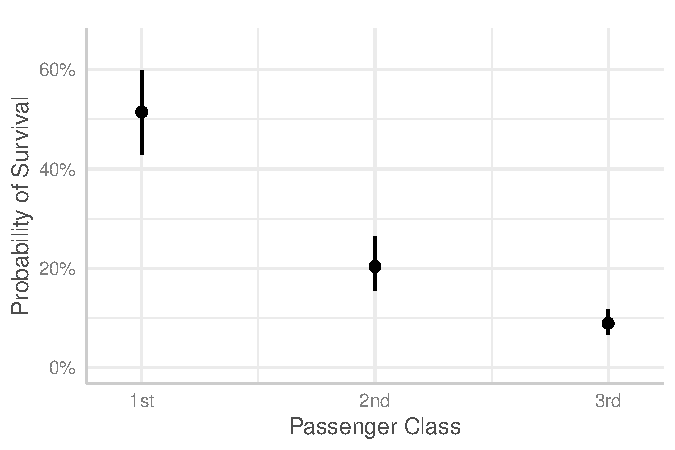
\includegraphics{group1_BenediktKronhardt_BorgeMeyer_files/figure-latex/pclass-ggeffects-1} 

}

\caption{Predicted probabilities of survival for each passenger class}\label{fig:pclass-ggeffects}
\end{figure}

Here, you can see another example to visualize the interaction between \texttt{sex} and \texttt{age}, that is, an interaction between a continuous and a categorical predictor.

\linespread{1}

\begin{Shaded}
\begin{Highlighting}[]
\NormalTok{eff2 }\OtherTok{\textless{}{-}} \FunctionTok{ggpredict}\NormalTok{(mlog1, }\AttributeTok{terms =} \FunctionTok{c}\NormalTok{(}\StringTok{"age [all]"}\NormalTok{, }\StringTok{"sex"}\NormalTok{))}
\FunctionTok{plot}\NormalTok{(eff2) }\SpecialCharTok{+} \FunctionTok{labs}\NormalTok{(}\AttributeTok{x =} \StringTok{"Age"}\NormalTok{, }\AttributeTok{y =} \StringTok{"Probability of Survival"}\NormalTok{,}
                  \AttributeTok{title =} \FunctionTok{element\_blank}\NormalTok{()) }\SpecialCharTok{+} 
    \FunctionTok{theme}\NormalTok{(}\AttributeTok{legend.position =} \StringTok{"bottom"}\NormalTok{) }\SpecialCharTok{+}
    \FunctionTok{guides}\NormalTok{(}\AttributeTok{color =} \FunctionTok{guide\_legend}\NormalTok{(}\AttributeTok{title =} \StringTok{"Sex"}\NormalTok{))}
\end{Highlighting}
\end{Shaded}

\linespread{1}

\begin{figure}[H]

{\centering 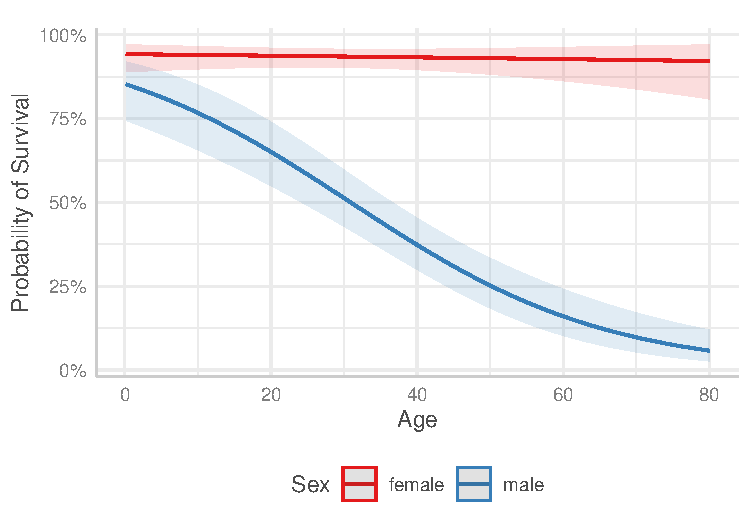
\includegraphics{group1_BenediktKronhardt_BorgeMeyer_files/figure-latex/sex-age-ggeffects-1} 

}

\caption{Predicted probabilities of survival dependend on sex and age}\label{fig:sex-age-ggeffects}
\end{figure}

Coming back to the multiple regression model from above (see section \ref{reg-models}), especially model 1 (see table \ref{tab:m123-modelsummary}), we can generate one visualization for all the main effects and one for the interaction. In a ``real'' scientific work you would not present the main effects for themselves in presence of an interaction involving these main effects, but for demonstration purposes, we want to generate four visualizations and put them together in one plot using the package \texttt{patchwork} (\protect\hyperlink{ref-Pedersen2022}{Pedersen 2022}). The code for this is placed on the following page, and the figure it produces comes on the next one. By the way, have a look into the chunk options for the last chunk, where both the arguments \texttt{fig.cap} and \texttt{fig.scap} are used to produce a caption and a short caption for figure \ref{fig:patchwork-plot}, where the former is printed under the figure itself and the latter is used in the list of figures to have a smaller output in the frontmatter.

\newpage

\linespread{1}

\begin{Shaded}
\begin{Highlighting}[]
\NormalTok{m1\_year }\OtherTok{\textless{}{-}} \FunctionTok{ggpredict}\NormalTok{(m1, }\AttributeTok{terms =} \StringTok{"year"}\NormalTok{)}
\NormalTok{m1\_cyl }\OtherTok{\textless{}{-}} \FunctionTok{ggpredict}\NormalTok{(m1, }\AttributeTok{terms =} \StringTok{"cyl"}\NormalTok{)}
\NormalTok{m1\_displ }\OtherTok{\textless{}{-}} \FunctionTok{ggpredict}\NormalTok{(m1, }\AttributeTok{terms =} \StringTok{"displ [all]"}\NormalTok{)}
\NormalTok{m1\_year\_cyl }\OtherTok{\textless{}{-}} \FunctionTok{ggpredict}\NormalTok{(m1, }\AttributeTok{terms =} \FunctionTok{c}\NormalTok{(}\StringTok{"cyl"}\NormalTok{, }\StringTok{"year"}\NormalTok{))}

\NormalTok{m1\_year\_plot }\OtherTok{\textless{}{-}} \FunctionTok{plot}\NormalTok{(m1\_year) }\SpecialCharTok{+} \FunctionTok{labs}\NormalTok{(}\AttributeTok{x =} \StringTok{"Year"}\NormalTok{, }
    \AttributeTok{y =} \StringTok{"Highway Miles per Gallon"}\NormalTok{, }\AttributeTok{title =} \FunctionTok{element\_blank}\NormalTok{()) }\SpecialCharTok{+} 
    \FunctionTok{scale\_y\_continuous}\NormalTok{(}\AttributeTok{limits =} \FunctionTok{c}\NormalTok{(}\DecValTok{0}\NormalTok{, }\ConstantTok{NA}\NormalTok{), }
                       \AttributeTok{breaks =} \FunctionTok{seq}\NormalTok{(}\AttributeTok{from =} \DecValTok{0}\NormalTok{, }\AttributeTok{to =} \DecValTok{50}\NormalTok{, }\AttributeTok{by =} \DecValTok{5}\NormalTok{))}
\NormalTok{m1\_cyl\_plot }\OtherTok{\textless{}{-}} \FunctionTok{plot}\NormalTok{(m1\_cyl) }\SpecialCharTok{+} \FunctionTok{labs}\NormalTok{(}\AttributeTok{x =} \StringTok{""}\NormalTok{, }
    \AttributeTok{y =} \StringTok{"Highway Miles per Gallon"}\NormalTok{, }\AttributeTok{title =} \FunctionTok{element\_blank}\NormalTok{()) }\SpecialCharTok{+} 
    \FunctionTok{scale\_y\_continuous}\NormalTok{(}\AttributeTok{limits =} \FunctionTok{c}\NormalTok{(}\DecValTok{0}\NormalTok{, }\ConstantTok{NA}\NormalTok{), }
                       \AttributeTok{breaks =} \FunctionTok{seq}\NormalTok{(}\AttributeTok{from =} \DecValTok{0}\NormalTok{, }\AttributeTok{to =} \DecValTok{50}\NormalTok{, }\AttributeTok{by =} \DecValTok{5}\NormalTok{))}
\NormalTok{m1\_displ\_plot }\OtherTok{\textless{}{-}} \FunctionTok{plot}\NormalTok{(m1\_displ) }\SpecialCharTok{+} \FunctionTok{labs}\NormalTok{(}\AttributeTok{x =} \StringTok{"Displacement"}\NormalTok{, }
    \AttributeTok{y =} \StringTok{"Highway Miles per Gallon"}\NormalTok{, }\AttributeTok{title =} \FunctionTok{element\_blank}\NormalTok{()) }\SpecialCharTok{+} 
    \FunctionTok{scale\_y\_continuous}\NormalTok{(}\AttributeTok{limits =} \FunctionTok{c}\NormalTok{(}\DecValTok{0}\NormalTok{, }\ConstantTok{NA}\NormalTok{), }
                       \AttributeTok{breaks =} \FunctionTok{seq}\NormalTok{(}\AttributeTok{from =} \DecValTok{0}\NormalTok{, }\AttributeTok{to =} \DecValTok{50}\NormalTok{, }\AttributeTok{by =} \DecValTok{5}\NormalTok{))}
\NormalTok{m1\_year\_cyl\_plot }\OtherTok{\textless{}{-}} \FunctionTok{plot}\NormalTok{(m1\_year\_cyl) }\SpecialCharTok{+} \FunctionTok{labs}\NormalTok{(}\AttributeTok{x =} \StringTok{""}\NormalTok{, }
    \AttributeTok{y =} \StringTok{"Highway Miles per Gallon"}\NormalTok{, }\AttributeTok{title =} \FunctionTok{element\_blank}\NormalTok{()) }\SpecialCharTok{+} 
    \FunctionTok{guides}\NormalTok{(}\AttributeTok{color =} \FunctionTok{guide\_legend}\NormalTok{(}\AttributeTok{title =} \StringTok{"Year"}\NormalTok{)) }\SpecialCharTok{+} 
    \FunctionTok{scale\_y\_continuous}\NormalTok{(}\AttributeTok{limits =} \FunctionTok{c}\NormalTok{(}\DecValTok{0}\NormalTok{, }\ConstantTok{NA}\NormalTok{), }
                       \AttributeTok{breaks =} \FunctionTok{seq}\NormalTok{(}\AttributeTok{from =} \DecValTok{0}\NormalTok{, }\AttributeTok{to =} \DecValTok{50}\NormalTok{, }\AttributeTok{by =} \DecValTok{5}\NormalTok{))}

\NormalTok{m1\_year\_plot }\SpecialCharTok{+}\NormalTok{ m1\_cyl\_plot }\SpecialCharTok{+}\NormalTok{ m1\_displ\_plot }\SpecialCharTok{+}\NormalTok{ m1\_year\_cyl\_plot }\SpecialCharTok{+}
    \FunctionTok{plot\_annotation}\NormalTok{(}\AttributeTok{tag\_levels =} \StringTok{\textquotesingle{}A\textquotesingle{}}\NormalTok{) }\SpecialCharTok{+}
    \FunctionTok{plot\_layout}\NormalTok{(}\AttributeTok{guides =} \StringTok{\textquotesingle{}collect\textquotesingle{}}\NormalTok{) }\SpecialCharTok{\&}
    \FunctionTok{theme}\NormalTok{(}\AttributeTok{legend.position =} \StringTok{\textquotesingle{}bottom\textquotesingle{}}\NormalTok{)}
\end{Highlighting}
\end{Shaded}

\linespread{1}

\begin{figure}[H]

{\centering 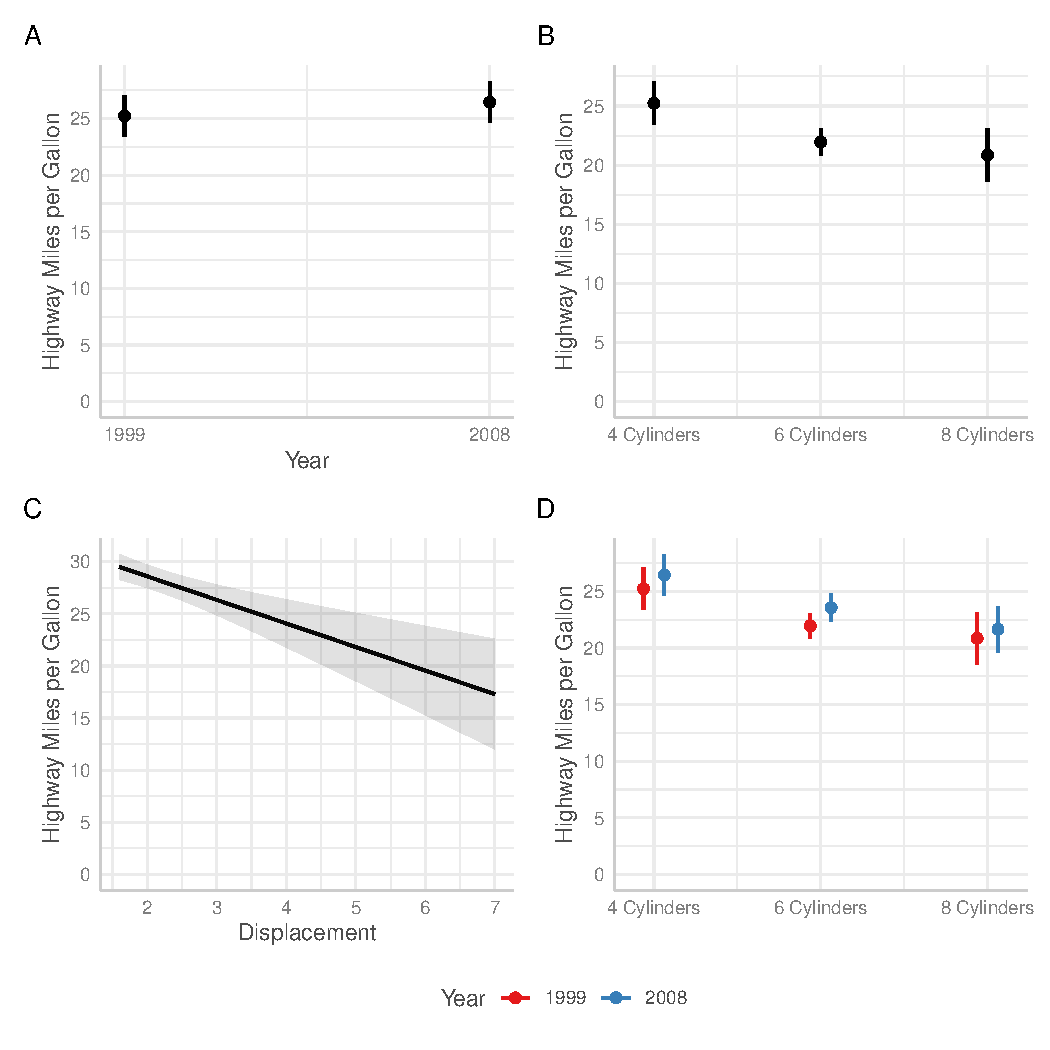
\includegraphics{group1_BenediktKronhardt_BorgeMeyer_files/figure-latex/patchwork-plot-1} 

}

\caption[One overall plot with four subplots]{One overall plot with four subplots: (A) predictor Year, (B) predictor Cylinders, (C) predictor Displacement, and (D) the interaction between Year x Cylinders}\label{fig:patchwork-plot}
\end{figure}

\begin{quote}
This is the end! Good luck with writing your own report or thesis using this template!
\end{quote}



\doublespacing

\end{document}
